\documentclass[12pt]{article}

%% Escrevendo em português
\usepackage[brazil]{babel}
\usepackage[utf8]{inputenc}
%\usepackage[latin1]{inputenc}
\usepackage[usenames,dvipsnames,svgnames,table]{xcolor}
\usepackage[a4paper,margin={1in}]{geometry}
\usepackage{graphicx}
\usepackage{indentfirst}
\usepackage{url}



%% Pulando linhas
\renewcommand{\baselinestretch}{2}

\newcommand{\vsp}{\vspace{0.2in}}
\newcommand{\etal}{{\it et al.}} 
\newcommand{\aluno}{{Carlos Eduardo Leão Elmadjian}}
\newcommand{\link}{\textit{link}} 
\newcommand{\links}{\textit{links}} 


\begin{document}
	
	\clearpage
	\thispagestyle{empty}
	
	\begin{minipage}[t]{6in}
		\begin{center}
			UNIVERSIDADE DE SÃO PAULO \\
			INSTITUTO DE MATEMÁTICA E ESTATÍSTICA\\
			DEPARTAMENTO DE CIÊNCIA DA COMPUTAÇÃO\\
			\vspace{5em}
			{\huge \textbf{Detecção de padrões de leitura com\\ baixa taxa de amostragem}}\\
			\vspace{2em}
			{\large \textbf{Trabalho de Formatura Supervisionado --- MAC0499}}\\
			\vspace{2em} 

		
			\vspace{8em}
			{\large \textbf{Aluno:} \aluno{}\\ }
			{\large \textbf{Orientador:} Prof. Dr. Carlos Hitoshi Morimoto\\}
			
			\vspace{5cm}
			\large{São Paulo, novembro de 2015}
		\end{center}
		
		
	\end{minipage}
	
	\vspace{150pt}
	
	
	\newpage
	
	\vsp
	
	
	\section*{Agradecimentos}
	Parece inevitável não cometer injustiças quando desejamos publicar nosso apreço por todos aqueles que contribuíram para nossa formação. Por isso, numa tentativa possivelmente canhestra de ser justo, restrinjo os agradecimentos apenas às pessoas que contribuíram especificamente para este trabalho.
	
	Agradeço, portanto, ao professor Hitoshi, pelo desafio, confiança, questionamentos e ensinamentos diretos e indiretos (que certamente não foram poucos).
	
	Aos amigos e colegas de laboratório, como o Adnan Degaki, que me deu algumas aulas sobre o \textit{Pupil Eye Tracker}, o Andrew Kurauchi (Toshi), que contribuiu imensamente com o protocolo experimental, o Fernando Aluani (Omar), que me forneceu dados valiosos de rastreamento, e tanto o Antonio Tula como o José Leyva, pelas frutíferas conversas.
	
	A todas as pessoas que se voluntariaram a dar cerca de 20 minutos do seu dia para um experimento sem nenhum tipo de recompensa pecuniária, apenas por amor à ciência ou consideração humanitária.
	
	Por fim, à Cintia Yamashita, minha companheira. Sem o seu apoio, compreensão e críticas, este trabalho não seria possível (a não ser numa versão decididamente pior e vexatória).
	
	Aos injustiçados, minhas sinceras desculpas e, novamente, muito obrigado.
	\clearpage
	
	%================================================================
	%SUMARIO
	\tableofcontents
	\clearpage
	
	%================================================================	
	\section{Resumo}
	
	Aplicações para computação vestível estão, potencialmente, sempre em funcionamento para auxiliar o usuário em tarefas cotidianas, porém esse estado de alerta constante pode ocasionar um alto consumo de energia e, ao mesmo tempo, prejudicar o usuário com interrupções indesejáveis. Dessa forma, é necessário que essas aplicações demandem poucos recursos da máquina e façam uso de contexto para melhorar a qualidade das interações. Neste trabalho, exploramos como o reconhecimento de padrões de leitura pode prover contexto para aplicações e quais abordagens algorítmicas podem ser empregadas para preservar energia por meio de soluções que trabalhem com baixa taxa de amostragem. Nossos resultados mostram que o algoritmo aqui proposto consegue manter o mesmo nível de desempenho em diferentes frequências, ao contrário de outros trabalhos na literatura.
	
	\vspace{1cm}
	\noindent \textbf{palavras-chave}: detecção de leitura, baixa taxa de amostragem, consumo de energia, computação vestível
	
	\clearpage
	
	
	%================================================================
	\section{Introdução}
	
		%------------------------------------------------------------
		\subsection{Motivação}
		Computadores cada vez menores e dedicados às mais diferentes tarefas, presos às nossas roupas, cabeça, olhos, ouvidos e pulsos. Esse cenário, que há décadas atrás não passaria de ficção científica, hoje se encontra cada vez mais próximo da realidade. 
		
		Contrário ao que intui o senso comum, os primeiros protótipos em computação vestível começaram a circular no meio acadêmico já desde a década de 1960 \cite{Sutherland-1968}. No entanto, o interesse na pesquisa por \textit{wearables} como uma nova maneira de interagir com computadores só ganhou verdadeiramente momento com os avanços tecnológicos no final da década de 1990 \cite{Mann-1997}.
		
		Idealmente, equipamentos vestíveis devem ser leves, resistentes, flexíveis, funcionar por um longo período de tempo e não devem monopolizar a atenção do usuário \cite{Mann-1997}. Além disso, muitos desses aparelhos não são de propósito geral, como os computadores tradicionais: cada um deles pode ser pensado para um fim que, grosso modo, está voltado para o auxílio do usuário em tarefas específicas do cotidiano. A somatória de todas essas características impõe novos paradigmas para como interagimos com a realidade \cite{Starner-2001}. Em particular, o uso de rastreadores de olhar como um acessório vestível já é aventado em pesquisas acadêmicas há alguns anos \cite{Bulling-2009} e representaria também uma nova maneira de interagir com computadores. 
		
		Embora os rastreadores façam parte de pesquisas científicas há quase um século, a maior parte dos estudos realizados com esses equipamentos esteve restrita à compreensão do comportamento ocular, algo de extremo valor para áreas como psicologia e neurociência. Já na ciência da computação, os rastreadores se tornaram objeto de estudo apenas mais recentemente, com os avanços tanto em poder computacional quanto em algoritmos para processamento de imagens \cite{Duchowski-2002}.
		
		As aplicações mais recorrentes de rastreadores dentro da ciência computação estão tradicionalmente ligadas à pesquisa de tecnologias assistivas, uma vez que certas condições médicas como Esclerose Lateral Amiotrófica (ELA), Síndrome do Encarceramento ou alguns tipos de tetraplegia subjugam seus portadores a uma limitação física extrema, de modo que só lhes restam os movimentos oculares como maneira exclusiva de interagirem com a realidade.
		
		Todavia, como tecnologia vestível, rastreadores ainda são pouco explorados. Apenas observando os principais tipos de movimentos dos olhos, como fixações (manutenção do olhar em uma região), sacadas (movimentos rápidos que duram entre 20 ms e 100 ms) e perseguições lentas, pode-se inferir sobre os interesses, preferências, dificuldades e outros comportamentos individuais \cite{Reichle-1998}. Embora já existam alguns trabalhos contemplando esses aspectos, não se encontram registros de como aplicar tais conhecimentos de modo contínuo no cotidiano das pessoas.
		
		Por fim, sendo a leitura hoje uma prática essencial na atividade humana, isto é, uma das habilidades mais relevantes para a qual as pessoas não foram biologicamente programadas \cite{Reichle-1998}, pouco se observa também na literatura a respeito de como a interpretação dos movimentos oculares podem prover pertinência aos usuários, como \textit{feedback} de relevância, assistência para interação sem as mãos, estatísticas para geração de conteúdo, entre outras possibilidades.
		
		%------------------------------------------------------------
		\subsection{Justificativa}
		
		Na literatura, alguns autores classificam a interação do olhar com interfaces de janelas em cinco diferentes tipos: inspeção, busca, exploração, monitoramento e leitura. Cada um desses tipos está associado a um padrão de comportamento, sendo a leitura, possivelmente, o mais relevante entre todos, isto é, aquele para o qual o usuário despende mais tempo e em que seu interesse se manifesta de forma mais clara \cite{Campbell-2001}.
		
		Por meio da análise da leitura em tempo real é possível depreender contexto: fixações prolongadas em uma região de um texto podem indicar dificuldade de compreensão de um termo, regressões constantes (e.g., releitura de uma linha) podem salientar uma dificuldade de compreensão geral, sacadas grandes sugerem falta de interesse sobre o conteúdo, enquanto que sacadas curtas alternadas com fixações rápidas indicam compenetração \cite{Rayner-1998}. Kunze et al. \cite{Kunze-2013} demonstraram que é possível, inclusive, inferir sobre o tipo de documento lido (e.g., revistas, jornais, quadrinhos) baseando-se apenas na análise dos padrões de leitura do usuário.
		
		Contudo, embora o estudo de algoritmos para detecção de leitura já tenha quase duas décadas \cite{Campbell-2001}, a investigação sobre como fazê-lo com baixa taxa de amostragem ainda é inédita e fundamenta-se, sobretudo, pelo fato de que o consumo de energia está rapidamente se tornando o fator limitante para dispositivos vestíveis \cite{Pouwelse-2001, Starner-2001}.
		
		Essa condição é ainda mais crítica para rastreadores de olhar móveis, que tipicamente apresentam ao menos duas câmeras --- uma para capturar o que o usuário enxerga (cena), e outra utilizada para capturar os movimentos oculares. Somando-se a isso o fato de os rastreadores de desempenho mais limitados hoje trabalharem a uma taxa de 30 Hz, o grau de processamento envolvido nessa quantidade de imagens por segundo está longe de ser desprezível, o que implica, consequentemente, um consumo de energia maior.
		
		Câmeras USB, quando em regime, podem ir de 100 mW de consumo (\textit{stand-by}) para até mais de 1000 mW \cite{Toms_Hardware}, tornando-se impróprias para o uso prolongado em dispositivos móveis, sobretudo em comparação com processadores desenvolvidos especificamente para equipamentos desse tipo, como a linha OMAP, da Texas Instruments, que tipicamente apresenta consumo inferior a 1000 mW \cite{OMAP}.

		O regime em potência baixa dos processadores também implica uma quantidade de cálculos por segundo inferior ao convencional para aplicações com grande consumo. Faz-se, portanto, necessário o emprego de técnicas que reduzam drasticamente a demanda sobre processamento das informações oriundas do olhar.
	
		%------------------------------------------------------------
		\subsection{Objetivos}
		O presente trabalho tem como objetivo central demonstrar uma solução para o problema da detecção de padrões de leitura com baixa taxa de amostragem, ensejando, dessa forma, aplicações de interesse público com rastreadores de olhar em computação vestível.
		
		Ainda dentro dessa meta, almejamos mostrar que, mesmo com tais condições restritivas, podemos estabelecer critérios de classificação do tipo de leitura (convencional ou \textit{skimming}), permitindo que futuras aplicações possam basear-se em contextos, ainda que rudimentares. 
		
		Como objetivos secundários, pretendemos exibir também um panorama das soluções existentes para reconhecimento da leitura por máquina e analisar problemas pertinentes à baixa taxa de amostragem de sinais para este propósito e, por fim, exibir uma prova de conceito do reconhecimento da leitura como mecanismo de contexto, utilizando o algoritmo desenvolvido ao longo desta investigação.
		
		%------------------------------------------------------------
		\subsection{Desafios}
		Os desafios para que o uso de contexto em computação vestível se expanda estão em pelo menos três frentes. Em primeiro lugar, há a questão da aceitação social no nível do \textit{hardware}: aparelhos invasivos, indiscretos, inseguros ou intrinsecamente sem propósito dificilmente terão algum impacto em termos de consumo de massa \cite{Mann-1998}. Sem o fomento apropriado, é possível que os investimentos e o interesse pela pesquisa na área entrem em declínio.
		
		Uma segunda frente a ser tratada está no nível das aplicações, e tal problema está intimamente ligado ao anterior, dado que uma massa crítica de desenvolvedores está associada a um panorama de oportunidades no setor \cite{Starner-2001}. Equipamentos potencialmente relevantes ao cotidiano do usuário são virtualmente inúteis sem aplicações que proporcionam ou facilitam alguma necessidade.
		
		O último e mais relevante desafio reside nos algoritmos. Desenvolver aplicações apropriadas, com um comportamento atento, passivo, inoportuno e, ao mesmo tempo, com \textit{consciência} de contexto, requer ainda uma pesquisa ampla na área de aprendizagem computacional das linguagens corporal e contextual humanas.
		
		Embora o padrão de leitura simples seja algo claramente discernível para um especialista, ainda assim é um sinal bastante ruidoso, e uma mera filtragem não é suficiente para eliminar --- ou somente mitigar --- esse ruído, uma vez que ele está associado não só ao indivíduo \textit{per se} como também à sua resposta comportamental ao conteúdo lido.
		
		Além disso, a leitura é tipicamente uma forma de interação não seletiva, ou seja, na qual o olhar não é empregado para o controle de uma interface. Portanto, não se deve presumir que o depreendimento das intenções do usuário nesse cenário seja equiparável às tomadas de decisões explicitamente mensuráveis em interações seletivas.
		
		Finalmente, poucos trabalhos têm tratado do uso desses padrões para novas formas de interação, tais como \textit{retorno de relevância}, como sugerido por Buscher et al. \cite{Buscher-2008} ou \textit{leitura aumetada}, como proposta por Biedert et al. \cite{Biedert-2010}. Interações mais sofisticadas (e possivelmente mais interessantes), considerando contextos com longos períodos de \textit{feedback} dos usuários e com o emprego de inteligência artificial sobre esses comportamentos, ainda carecem de investigação.
		\clearpage
	
	%================================================================	
	\section{Características da leitura}
	
		%------------------------------------------------------------
		\subsection{O movimento do olhar na leitura}
		Para que se possa dissertar sobre como o olhar se comporta na leitura, é preciso antes definir o que de fato denotamos como leitura. Neste trabalho, esse termo tem um significado muito mais preciso do que se pode inicialmente supor.
		
		Em primeiro lugar, este estudo trata da leitura de textos em línguas indo-europeias em que a ordem com que se percorre os caracteres da escrita se dá da esquerda para a direita (primariamente) e de cima para baixo (secundariamente). Isso pode soar um tanto trivial para leitores ocidentais, mas essa ressalva é fundamental: em algumas línguas asiáticas, como chinês, japonês ou coreano, a convenção do sentido de leitura é da direita para esquerda. O mesmo vale também para línguas do Oriente Médio, com o intrigante fato de que em línguas arábicas é praxe escrever termos estrangeiros da esquerda para direita, o que pode tornar o sentido da leitura um tanto confuso em alguns casos.
		
		Ademais, quando nos referimos à leitura, estamos tratando do comportamento dito \textit{convencional}, segundo a literatura \cite{Pavlidis-1981}, isto é, excluímos aqui todas as outras manifestações de leitura que representam uma anomalia frente a esse padrão (Figura \ref{fig:dyslexia}), como a de indivíduos portadores de dislexia, portadores do Transtorno do Déficit de Atenção e Hiperatividade (TDAH), crianças em estágio inicial de alfabetização ou mesmo adultos semialfabetizados.
		
		\begin{figure}[!ht]
			\centering
			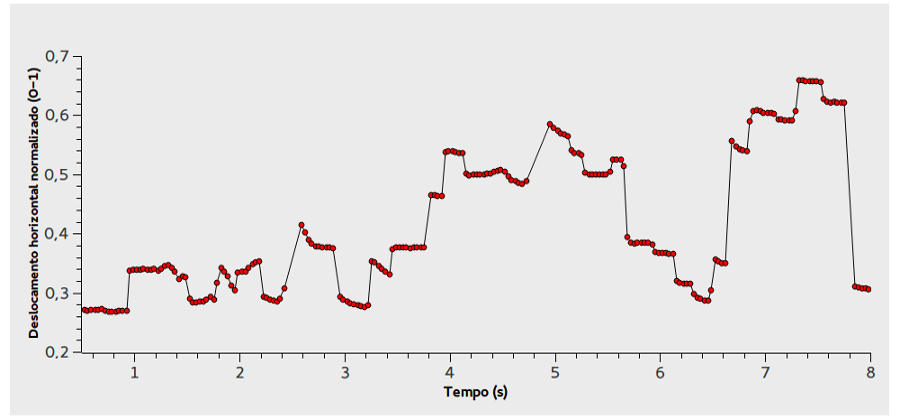
\includegraphics[width=14cm]{imgs/leitura_horizontal2.png}
			\caption{\footnotesize {O padrão de um indivíduo clinicamente diagnosticado com TDAH. Nesse caso, as perturbações causadas por regressões são frequentes, o que dificulta a identificação do comportamento de leitura.}}
			\label{fig:dyslexia}
			\vspace{5mm}
		\end{figure}
		
		Feitas as devidas ressalvas, podemos caracterizar a leitura, em termos do movimentos oculares, como uma alternância entre sacadas e pequenas fixações com 200 a 300 ms de duração, sendo essas sacadas tipicamente curtas e feitas predominantemente da esquerda para a direita ao longo de uma linha de texto. Quando se atinge o fim da linha, o olho faz uma nova sacada, muito maior, em geral, para o início da próxima linha, um deslocamento comumente denominado de \textit{regressão}, termo que também pode ser empregado para classificar movimentos de releitura \cite{Rayner-2001}.
		
		Durante as sacadas, os olhos se movem a mais de 500$^o$ por segundo, quando então ocorre a \textit{supressão sacádica}, isto é, não é possível obter informação visual distinta da cena \cite{Rayner-1998}, razão pela qual o cérebro só consegue extrair informações de um texto durante fixações.
		
		Todavia, embora o campo de visão humano seja de aproximadamente 180$^o$, só temos acuidade visual em uma pequena região da imagem que capturamos da cena (Figura \ref{fig:acuidade}). Isso porque a percepção dos detalhes é uma propriedade dos cones, células fotossensíveis que se concentram apenas numa região específica da retina, denominada fóvea, que se localiza no centro do eixo ótico. Assim, o conjunto de fixações realizadas durante a leitura se distribui ao longo das linhas de um texto de forma a criar uma cobertura das informações com o máximo possível de acuidade.
		
		\begin{figure}[!ht]
			\centering
			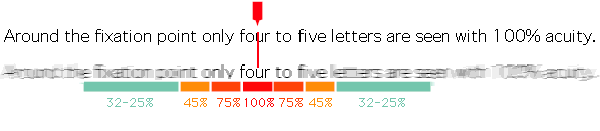
\includegraphics[width=14cm]{imgs/acuidade.png}
			\caption{\footnotesize {Representação artística da acuidade visual humana quando uma imagem é capturada durante uma fixação. O ponteiro vermelho indica o centro do eixo ótico, alinhado com a fóvea. \cite{Acuidade}}}
			\label{fig:acuidade}
			\vspace{5mm}
		\end{figure}
		
		Outros movimentos oculares, como vergência, vestibular e perseguição, contribuem muito pouco para caracterizar a leitura, sobretudo dentro do modelo clássico de análise, em que se supõe textos a uma distância fixa, com o leitor relativamente inerte \cite{Lee-1999}. Se construirmos um gráfico dos movimentos horizontais do olho durante a leitura em função do tempo, percebemos uma padrão muito claro (Figura \ref{fig:staircase}), dependente basicamente de fixações e sacadas, que por sua vez é conhecido na literatura como \textit{staircase pattern} \cite{Lee-1999}. 
		
		\begin{figure}[!ht]
			\centering
			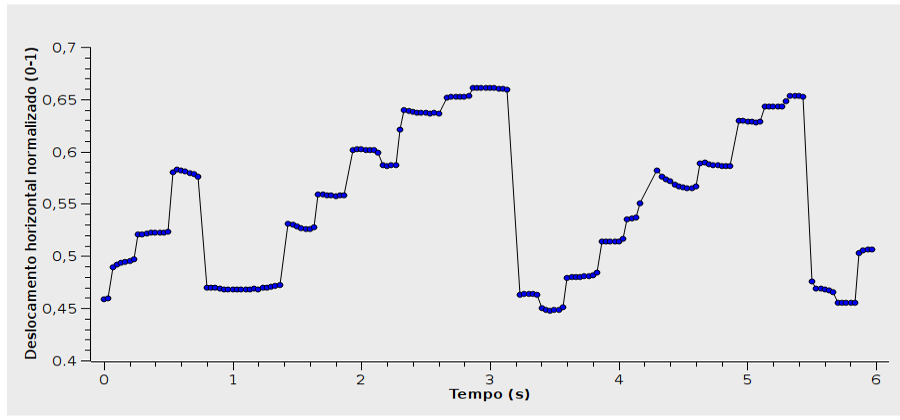
\includegraphics[width=14cm]{imgs/leitura_horizontal1.png}
			\caption{\footnotesize {O \textit{staircase pattern} de um leitor clinicamente saudável. Note que podem ocorrer movimentos de releitura, mas eles não são predominantes no comportamento.}}
			\label{fig:staircase}
			\vspace{5mm}
		\end{figure}
		

		
		%------------------------------------------------------------
		\subsection{Depreendimentos do comportamento de leitura}
		Durante a chamada \textit{segunda era} das pesquisas com rastreadores de olhar, marcadas pelas investigações behavioristas, surgiram os primeiros trabalhos que registraram os movimentos característicos do olhar na leitura \cite{Duchowski-2002}. No entanto, somente em meados de 1970 é que se passou a estudar mais intensamente as implicações cognitivas do processo de leitura \cite{Rayner-1998}.
		
		Os primeiros trabalhos nesse sentido pressupunham que leitores proficientes faziam um significativo uso do contexto textual para conseguir processar informações rapidamente. Embora essa concepção tenha sido validada empiricamente, estudos posteriores mostraram que o uso do contexto é ainda mais relevante para leitores iniciantes \cite{Rayner-2001}.
		
		De todo modo, a familiaridade de indivíduos com um texto é algo sobre o que se pode inferir a partir dos movimentos oculares. Leitores proficientes, em geral, dependem menos da região de grande acuidade visual do que principiantes para capturar informações. Acredita-se que a experiência pessoal gradualmente forneça um arcabouço de inferências baseadas em contexto. Dessa forma, leitores experientes podem, por exemplo, ler apenas os três primeiros caracteres de uma palavra para processá-la e utilizar informações periféricas à região de acuidade, como o tamanho do próximo termo, para realizar suposições baseadas em contexto semântico \cite{Rayner-1998, Rayner-2001}.
		
		Outro fator relevante sobre processos cognitivos a partir dos movimentos do olhar na leitura é o tempo de fixação. Já se constatou em experimentos que passagens de texto consideradas difíceis geram, em média, tempos de fixação maiores nos leitores. Em geral, termos raros, desconhecidos ou contextualmente inapropriados recebem, por exemplo, um tempo maior de atenção do leitor em contraste com a média \cite{Reichle-1998}.
		
		Finalmente, podemos inferir características do leitor baseando-nos no conjunto de sacadas acumuladas ao longo de um determinado tempo. Indivíduos com alfabetização precária ou com déficit de atenção costumam apresentar um padrão de regressões constantes, ou seja, termos, linhas ou mesmo parágrafos são relidos com uma frequência atípica (Figura \ref{fig:dyslexia}) \cite{Pavlidis-1981, Rayner-1998}. Por outro lado, poucas fixações por linha, intercaladas por sacadas espaçadas, podem insinuar pressa, busca por informação ou desinteresse do leitor \cite{Dyson-2001}.
			
		
		
		%------------------------------------------------------------
		\subsection{Diferenças entre leitura e \textit{skimming}}
		Se por um lado há um consenso no meio acadêmico sobre o que caracteriza a leitura convencional, por outro, não há um entendimento claro quanto à classificação da leitura rápida. Alguns autores subdividem essa atividade em dois grupos (\textit{skimming} e \textit{scanning}) \cite{Campbell-2001}, enquanto outros julgam que a partir de um determinado limiar de palavras por minuto, tudo que se assemelhe à leitura deve ser entendido como \textit{skimming} \cite{Rayner-1998}.
		
		O limiar mais aceito, nesse caso, está entre 600 - 700 palavras por minuto e foi estabelecido empiricamente \cite{Rayner-1998}. Dado que um leitor proficiente lê, em média, a uma taxa de 250 palavras por minuto, intui-se que com mais do que o dobro da velocidade haja uma queda significativa da compreensão do texto.
		
		Alguns estudos, porém, revelaram que embora haja uma correlação forte entre o nível de compreensão do indivíduo e a taxa de leitura, ainda assim é possível capturar as principais informações de um texto lendo-se rapidamente, de modo a se preservar um bom entendimento do conteúdo, em detrimento, é claro, dos detalhes. Curiosamente, observou-se ainda que a taxa de compreensão é ótima quando o indivíduo se sente levemente pressionado e lê a uma velocidade um pouco acima do que considera normal \cite{Dyson-2001}. 
		
		Portanto, mesmo sem uma definição precisa, existe um entendimento de que a atividade de \textit{skimming} certamente não é algo excêntrico à leitura. Embora seja mecanicamente impossível para um ser humano ler a mais de 600 palavras por minuto (dadas as latências de preparação de sacadas, fixações e movimentos de estabilização do olho \cite{Reichle-1998}), a literatura mostra que o \textit{skimming} é claramente distinto, por exemplo, de uma busca rápida por uma palavra em um texto.
		
		Por outro lado, o \textit{skimming} não é exatamente uma leitura acelerada. A uma velocidade entre 600 - 700 palavras por minutos, um indivíduo deixa de capturar várias informações que estão fora do seu campo de acuidade visual, o número de fixações por linha é menor, a latência das fixações é menor e o contexto desempenha um papel ainda mais significativo no entendimento, isto é, o cérebro acaba preenchendo com suposições semânticas o vazio deixado pela falta de dados visuais \cite{Rayner-1998}.
		
		
		
		%------------------------------------------------------------
		\subsection{Reconhecimento de leitura por máquina}
		Ainda que a leitura tenha um padrão característico, tal padrão está longe de uma natureza determinística. A leitura está intimamente ligada à cognição humana \cite{Rayner-1998}, um processo complexo e alimentado por diversos componentes como influências do ambiente, experiências pessoais, formação educacional, contexto textual, saúde, entre outros. Portanto, embora emerja uma ordem desse aparente caos, trata-se de uma ordem relativamente ruidosa \cite{Lee-1999}.
		
		Para que uma máquina possa reconhecer se uma pessoa está lendo a partir dos seus movimentos oculares, precisamos eliminar --- ou pelo menos mitigar --- esse ruído. Entretanto, essa não é uma tarefa simples. 
		
		Consideremos o modelo do movimento de leitura idealizado em comparação com um conjunto de dados coletados na prática (Figura \ref{fig:idealizado}). Não é difícil perceber a semelhança entre ambos, mas também não se deve supor que há um padrão no ruído. Um indivíduo pode reler o mesmo texto de diferentes maneiras, fazendo fixações com latências distintas para as mesmas regiões, sacadas de diferentes tamanhos, releituras ou saltos, imprevisivelmente. Tudo depende do processo cognitivo, algo essencialmente subjetivo.
		
		\begin{figure}[!ht]
			\centering
			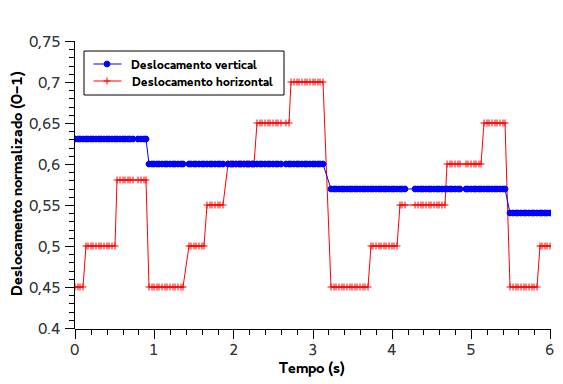
\includegraphics[width=7.8cm]{imgs/idealizado_1.png}
			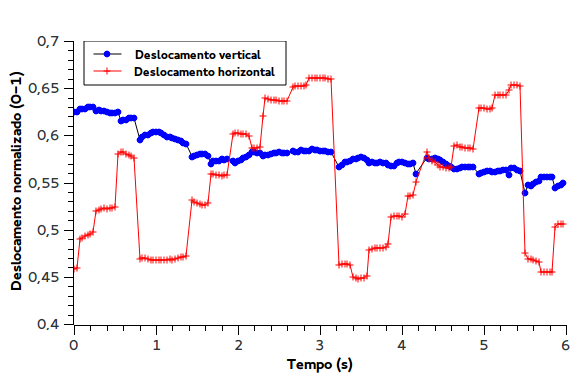
\includegraphics[width=7.8cm]{imgs/idealizado_2.png}
			\caption{\footnotesize {À esquerda, o modelo idealizado do padrão de leitura: as fixações ocorrem dentro de um intervalo limitado e os deslocamentos horizontal e vertical são uniformes. À direita, o padrão de leitura real de um indivíduo.}}
			\label{fig:idealizado}
			\vspace{5mm}
		\end{figure}

		Mesmo entre leitores proficientes, o modelo idealizado está longe de ser perfeito. Estima-se que 10\% do tempo seja gasto com regressões \cite{Reichle-1998} e vários estudos exibem evidências de que esses leitores conseguem deduzir palavras subsequentes em algumas circunstâncias, mesmo quando tais termos não se encontram na sua região de alta acuidade visual, o que permite que façam menos fixações por linha \cite{Rayner-2001}, distorcendo o poder de previsão do modelo.
		
		Como se isso não bastasse, deve-se considerar que a cabeça dificilmente permanece rígida enquanto lemos. Logo, os movimentos de tronco e cabeça durante a leitura fazem com que as fixações apresentem um caráter de instabilidade \cite{Lee-1999}, sendo impregnadas por movimentos vestibulares e de estabilização do globo ocular.
		
		Dessa forma, parece razoável supor que uma abordagem estatística para detectar o evento de leitura seja o caminho mais adequado para o reconhecimento de máquina. De fato, essa percepção é corroborada pela literatura, uma vez que todos os algoritmos para reconhecimento de padrões de leitura publicados até então utilizam estratégias probabilísticas, como veremos na próxima seção.
		\clearpage
		
	%================================================================
	\section{Algoritmos}
	
		Nesta seção, iremos tratar dos principais algoritmos presentes na literatura para reconhecimento da leitura a partir de rastreadores de olhar. Vamos fazer uma descrição geral sobre seu funcionamento e discutir brevemente os resultados alcançados pelos autores.  
	
		%------------------------------------------------------------
		\subsection{Algoritmo de Campbell e Maglio (2001)}
		Campbell e Maglio foram os primeiros autores na literatura a proporem, especificamente, um algoritmo para detecção de leitura por máquina. Sua solução fundamenta-se no reconhecimento de eventos do olhar e na subsequente classificação desses eventos de acordo com um modelo idealizado de leitura \cite{Campbell-2001}.
		
		Para viabilizar o processo em tempo real, é construída uma representação simplificada dos movimentos do olhar, de maneira que os únicos eventos a serem detectados sejam fixações e sacadas. Para o bom funcionamento do algoritmo, são necessárias ainda algumas condições de controle, como uma postura rígida do leitor em relação ao texto, uma distância fixa pré-determinada e o conhecimento prévio do tamanho dos caracteres a serem lidos.
		
		O método consiste em usar as coordenadas do olhar transformadas para um plano em intervalos de 100 ms, coletando-se 60 pontos por segundo. Para suavizar erros inerentes à função de calibração e minimizar perturbações involuntárias do usuário, os autores sugerem o emprego da média de três pontos adjacentes, totalizando, então, 20 pontos médios por segundo.
		
		A ideia central é acumular \textit{evidências de leitura} em uma variável sempre que o olho fizer um movimento favorável ao modelo de leitura e decrementar o valor dessa variável quando o olho realizar um movimento contrário. No total, os autores definem 13 tipos de eventos vindos do rastreador a serem interpretados (Tabela \ref{tab:campbell_tab}), todos em função de eixo, distância e direção do olhar. Os eventos são então ``tokenizados'' e recebem uma pontuação de acordo com o \textit{token}.
		
		\begin{table}[!h]
			\renewcommand{\arraystretch}{0.8}
			\begin{center}
				\begin{tabular}{|p{6cm}|l|c|}  \hline
					\textbf{eixo, distância e direção} & \textbf{Token} & \textbf{Pontuação}\\\hline
					X curto à direita  & leitura   & 10  \\
					X médio à direita  & \textit{skimming}  & 5  \\
					X longo à direita  & \textit{scanning}  & \textit{Reset} \\
					X curto à esquerda & regressão & -10 \\
					X médio à esquerda & \textit{skimming}  & -5  \\
					X longo à esquerda & \textit{scanning}  & \textit{Reset}  \\
					Y curto para cima  & \textit{skimming}  & -5 \\
					Y médio para cima  & \textit{scanning}  & \textit{Reset} \\
					Y longo para cima  & \textit{scanning}  & \textit{Reset}  \\
					Y curto para baixo & sacada antecipatória & 0  \\
					Y médio para baixo & \textit{skimming} & -5\\
					Y longo para baixo & \textit{scanning} & \textit{Reset}\\
					X longo ou médio para esquerda + Y curto para baixo & reinício de linha & 5\\\hline
					
				\end{tabular}
			\end{center}
			\label{tab:campbell_tab}
			\caption{\footnotesize{Esquema de pontuação de Campbell e Maglio por ``tokenização'' de movimentos do olhar. A pontuação positiva indica evidências de suporte à leitura, enquanto a negativa sinaliza o contrário.}}
		\end{table}
		
		Para que a leitura seja detectada, a pontuação acumulada (com múltiplos de cinco) deve ultrapassar um limiar de valor 30, determinado heuristicamente por Campbell e Maglio. Esse limiar também é fundamental para tratar dos problemas atrelados ao ruído do sinal, uma vez o sistema só deve reconhecer o comportamento de leitura com um conjunto significativo de indícios.		
		
		Em termos de desempenho, o algoritmo, de acordo com os autores, apresentou uma acurácia superior a 90\%, algo não reprodutível em nossos experimentos. Contudo, o índice de falsos positivos pôde ser verificado empiricamente. Deve pesar ainda o fato de que não tivemos acesso aos mesmos equipamentos, tampouco pudemos trabalhar com o mesmo patamar de amostragem da publicação.
		
		%------------------------------------------------------------
		\subsection{Algoritmo de Buscher et al. (2008)}
		O algoritmo de Buscher et al.\cite{Buscher-2008} representa, de certo modo, uma sofisticação do algoritmo de Campbell e Maglio (2001). Trata-se também de um dos poucos trabalhos na literatura que procura reconhecer não apenas a leitura como também o padrão de \textit{skimming}.
		
		A metodologia adotada é semelhante à de Campbell e Maglio, mas também há novos mecanismos de robustez. O primeiro deles é a detecção de fixações: no lugar de usar uma mera suavização de pontos do olhar, o algoritmo procura coletar amostras suficientes para determinar se o usuário está realizando uma fixação. Isso é feito delimitando-se um quadrado de tolerância sobre a superfície observada, de modo que todos os pontos próximos o bastante que recaiam sobre o quadrado são considerados partes de uma mesma fixação. Se mais de três pontos consecutivos não pertencerem a essa região, então a fixação terminou.
		
		Uma outra melhoria está no uso de uma ferramenta de reconhecimento óptico de caracteres (OCR) do texto lido para parametrizar o algoritmo em função do espaço ocupado por letras. Como a caracterização das transições do olhar é bastante dependente do entrelinhamento e do tamanho da fonte do texto, obtém-se assim um esquema mais robusto de medição. Ademais, tais transições são medidas entre os baricentros das fixações.
		
		Embora aparente ser mais complexo que o de Campbell e Maglio, o algoritmo traz uma simplificação importante: os eventos a serem detectados agora são sete em vez de 13 (Tabela \ref{tab:buscher_tab}). Novamente, o roteiro é semelhante à solução anterior: os eventos reconhecidos são ``tokenizados'' e cada \textit{token} recebe uma pontuação. A diferença está no fato de que os mesmos \textit{tokens} também são usados para contabilizar evidências para o \textit{skimming} --- com esquema de pontuação distinto, é claro. Assim, se o algoritmo coleta um conjunto de evidências que ultrapasse o valor 30, a leitura passa a ser detectada. Para o caso do \textit{skimming}, o valor é 20. 
		
		\begin{table}[!h]
			\begin{center}
				\renewcommand{\arraystretch}{0.9}
				\begin{tabular}{|p{5cm}|l|p{2.5cm}|p{2.5cm}|}  \hline
					\textbf{Distância e direção em espaço de letras} & \textbf{Token} & \textbf{Pontuação leitura} & \textbf{Pontuação \textit{skimming}}\\\hline
					$0 < X <= 11$   & leitura   & 10       & 5\\
					$ 11 < X <= 21$ & \textit{skimming}  & 5        & 10\\
					$21 < X <= 30$  & \textit{skimming} longo  & -5  & 8\\
					$-6 <= X < 0$   & regressão curta & -8 & -8\\
					$-16 <= X < -6$ & regressão longa & -5 & -3\\
					$X < -16$ e Y curto-baixo& reinício de linha & 5& 5\\
					Outros movimentos  & não relacionado  & 0 & 0\\\hline
					
				\end{tabular}
			\end{center}
			\label{tab:buscher_tab}
			\caption{\footnotesize{Esquema de pontuação de Buscher et al. As transições entre uma fixação e a seguinte são classificadas em \textit{tokens} e uma pontuação correspondente é atribuída, podendo sinalizar dois estados: leitura ou \textit{skimming}.}}
		\end{table}
		
		Pelo fato de o algoritmo não ser o foco principal do artigo, Buscher et al. não exibem resultados de desempenho, como precisão e revocação. De todo modo, nossos experimentos mostraram que o algoritmo tem um comportamento compatível com o relatado no caso de Campbell e Maglio \cite{Campbell-2001} a uma taxa de 30 Hz.
		
				
		%------------------------------------------------------------
		\subsection{Algoritmo de Kollmorgen e Holmqvist (2007)}
		Este algoritmo \cite{Kollmorgen-2007}, assim como os demais apresentados nesta seção, utiliza um modelo do comportamento do olhar na leitura para detectá-la. A diferença, porém, reside no fato de que as alternâncias entre fixações e sacadas são representadas por um Modelo Oculto de Markov (HMM).
		
		A primeira fase do algoritmo é de pré-processamento dos dados: deve-se analisar todos os pontos do olhar coletados e eliminar todos os movimentos que não sejam fixações ou sacadas. Piscadas também são computadas nesse processo e cada fixação é armazenada numa estrutura de dados contendo sua posição espacial, tempo de início e duração. Já as sacadas são contabilizadas como segmentos entre duas fixações.
		
		Concluída essa fase, inicia-se a construção de uma máquina de estados finita, em que as transições e a saída são probabilísticas. Kollmorgen e Holmqvist acreditam que a leitura pode ser bem descrita por um HMM com seis estados e duas partições: leitura e não leitura (Figura \ref{fig:kollmorgen}). Definido o modelo e os parâmetros iniciais, os estados mais prováveis de transição são calculados a partir do algoritmo de Viterbi \cite{Rabiner-1989}.
		
		\begin{figure}[!ht]
			\centering
			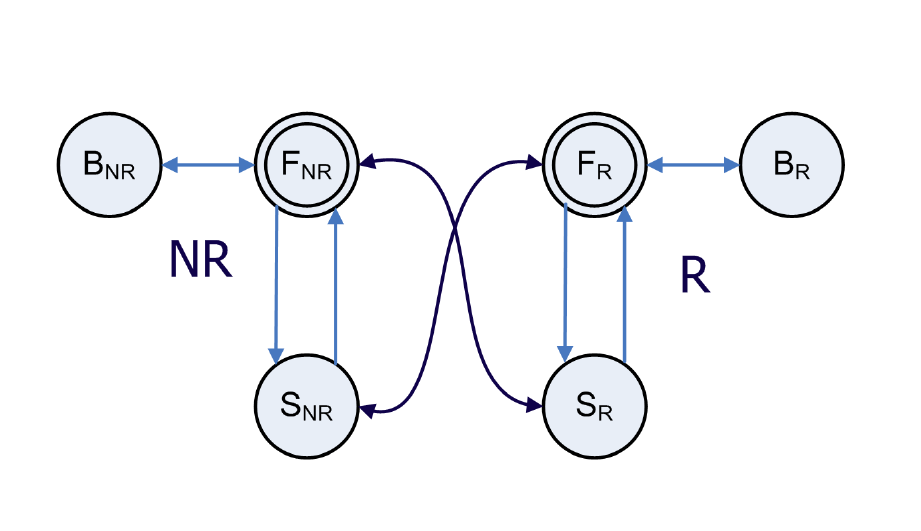
\includegraphics[width=10cm]{imgs/kollmorgen.png}
			\caption{\footnotesize {Modelo markoviano de Kollmorgen e Holmqvist. \textbf{R} indica leitura e \textbf{NR}, não leitura. Os estados \textbf{B}, \textbf{F} e \textbf{S} representam piscadas, fixações e sacadas, respectivamente.}}
			\label{fig:kollmorgen}
			\vspace{5mm}
		\end{figure}
		
		Os autores argumentam que a tarefa mais complexa no algoritmo é determinar os parâmetros para o modelo. Um método proposto é analisar previamente o conjunto de dados e tentar realizar o \textit{fitting}, isto é, utilizando supervisão. Eles também demonstram que é possível procurar os parâmetros de maneira não supervisionada, mas com resultados significativamente piores ($<$80 \%).		
		
		Embora os autores relatem que o algoritmo possa ser executado em tempo real, o artigo condiciona toda execução a um pré-processamento intenso de dados e treinamento, o que de certa maneira contraria essa alegação. Somando-se a isso o fato de que a solução não apresenta um desempenho equiparável ao dos demais, tampouco uma complexidade computacional baixa, optamos por não implementá-la, pois não poderia posteriormente ser adaptada como uma alternativa eficiente e de baixo consumo para reconhecimento de padrões de leitura.   
		
		\clearpage
	%================================================================
	\section{Estudo da baixa taxa de amostragem}
		
		%------------------------------------------------------------
		\subsection{A frequência de Nyquist}
		O Teorema da Amostragem de Nyquist-Shannon é uma das ferramentas fundamentais em processamento digital de sinais (DSP). A sua definição mais recorrente, atribuída a Shannon, é dada da seguinte forma: ``Se uma função $f(t)$ não contém frequências maiores do que $W$ Hz, então ela pode ser completamente determinada por suas ordenadas em uma série de pontos espaçados $\frac{1}{2}W$ segundos'' \cite{Shannon-1949}.
		
		Em outras palavras, o teorema estabelece que se quisermos representar um sinal adequadamente, precisamos registrar pelo menos metade da sua frequência máxima. Caso contrário, a reconstrução da função se torna ambígua, ocorrendo o fenômeno denominado \textit{aliasing} (Figuras \ref{fig:aliasing} e \ref{fig:aliasing2}).
		
		\begin{figure}[!ht]
			\centering
			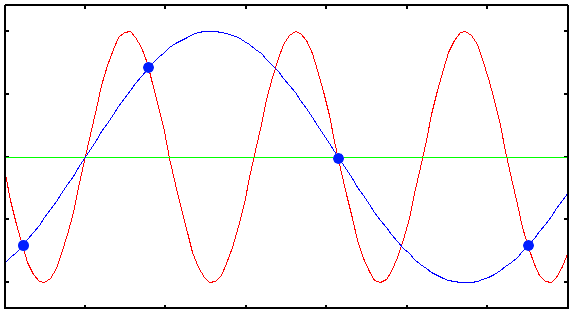
\includegraphics[width=10cm]{imgs/aliasing_one_dim.png}
			\caption{\footnotesize {Exemplo de \textit{aliasing} de uma senoide em função do tempo: a amostragem dada pelos pontos azuis não permite reconstruir corretamente o sinal original, em vermelho.}}
			\label{fig:aliasing}
			\vspace{5mm}
		\end{figure}
		
		\begin{figure}[!ht]
			\centering
			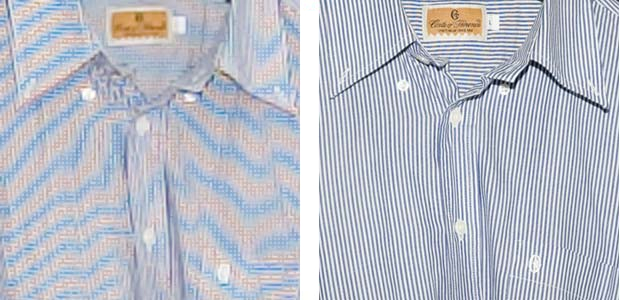
\includegraphics[width=16cm]{imgs/aliasing_image.jpg}
			\caption{\footnotesize {O fenômeno de \textit{aliasing} também pode ocorrer em duas dimensões, como no caso de imagens. Nesse caso, temos uma função de distância com duas variáveis, mas os efeitos da subamostragem (imagem à esquerda) estão relacionados ao caso de uma variável.}}
			\label{fig:aliasing2}
			\vspace{5mm}
		\end{figure}  
		
		O teorema se torna particularmente relevante em nosso caso, uma vez que computadores são máquinas de aritmética finita e, portanto, não possuem memória ilimitada para representar de modo contínuo um sinal capturado. Utilizando o teorema, intuímos que talvez seja possível reconstruir esse sinal de maneira discreta, conhecendo a quantidade mínima de amostras para isso \cite{Jerri-1977}. A resposta para essa intuição está na \textit{frequência de Nyquist}.
		
		De certo modo, a frequência de Nyquist é uma concessão à impossibilidade de se representar funções contínuas com DSP: dado que não é possível adquirir infinitas amostras de um sinal contínuo, estabelece-se que para representar uma quantidade de $S$ amostras por segundo devemos capturar pelo menos $\frac{1}{2}S$ amostras igualmente espaçadas no mesmo intervalo \cite{Grenander-1959}.
		
		Na prática, essa limitação muitas vezes é imperceptível, já que há várias evidências de que a percepção humana também se dá de maneira discreta \cite{VanRullen-2003}. Assim, com uma representação suficientemente fina de um sinal (seja ele uma imagem ou um som, por exemplo), podemos provocar a ilusão da percepção de um sinal contínuo, desde que a frequência de \textit{Nyquist} seja respeitada. 
		
		%------------------------------------------------------------
		\subsection{Padrões do olhar e o número de amostras}
		A maioria dos rastreadores de olhar empregados em trabalhos na literatura funciona a uma taxa de 50 a 60 imagens da pupila por segundo, uma frequência considerada adequada o suficiente para capturar interações do olhar com telas de computador \cite{Goldberg-1999}. 
		
		Considerando que uma fixação típica para a aquisição de informação dura entre 200 e 300 ms \cite{Rayner-1998, Goldberg-1999}, então um sistema de rastreamento em regime de 60 Hz poderá coletar em torno de 12 a 18 amostras desse evento. No entanto, é possível que ocorram fixações rápidas durante a interação, mas, em geral, com duração não inferior a 100 ms, o que nos leva a um mínimo de seis amostras para a detecção de uma fixação com esse equipamento.
		
		Já as sacadas são movimentos muito rápidos e de baixa duração (entre 20 e 100 ms \cite{Rayner-1998, Reichle-1998}). Detectá-las a 60 Hz ainda é possível (teríamos de uma a cinco amostras), mas identificá-las como tal seria algo um pouco mais complexo. Isso porque para os casos em que tivermos menos de três amostras, não há como garantir se os pontos coletados são, por exemplo, \textit{outliers}, frutos de um erro de calibração. 
		
		Os movimentos de perseguição, por outro lado, não possuem uma duração definida, mas por apresentarem velocidade e amplitude menores que as sacadas, podem ser percebidos por um sistema de rastreamento com base na direção e deslocamentos realizados pela pupila (\textit{scanpath}). 
		
		Outros movimentos mais sutis (de estabilização, por exemplo) também podem ser detectados, porém costumam estar associados a outros, como fixações. Além disso, a amostragem pode sofrer influência de ruídos inerentes ao processo de rastreamento, como movimentos involuntários de tronco e cabeça, no caso de rastreadores remotos, erros da função de calibração e o desalinhamento do centro da pupila em relação à fóvea.
		
		Neste trabalho, iremos realizar nossas análises com um rastreador de 30 Hz vestível \cite{Kassner-2014}. Sendo assim, teremos acesso a apenas metade das amostras mínimas aqui contabilizadas e a identificação de sacadas poderá ficar prejudicada. Para efeito de investigação, todavia, essa restrição é irrelevante, dado que, a rigor, todos os algoritmos para reconhecimento de leitura identificam as sacadas por meio da diferença entre fixações.
		
		%------------------------------------------------------------
		\subsection{Resolução mínima para detecção da pupila}
		O reconhecimento da pupila, embora não seja o foco deste trabalho, desempenha um papel fundamental no escopo do problema: se quisermos aplicações de longa duração para dispositivos vestíveis, essas aplicações devem demandar o menor consumo de processamento possível, mantendo um nível de usabilidade satisfatório.
		
		Quanto melhor a resolução da imagem da pupila, maiores são as chances de um sistema reconhecedor mapear corretamente o centro da pupila para um ponto em uma tela, por exemplo. Contudo, o custo do processamento de imagens cresce, no mínimo, quadraticamente em função do tamanho, dado que elas são representadas computacionalmente como uma matriz de \textit{pixels}, em que que cada coordenada armazena uma certa quantidade de valores --- a depender do modelo de cor adotado, como RGB, RGBA, HSV, escala de cinza, entre outros.
		
		Não há ainda na literatura trabalhos que mostrem quais as condições mínimas de resolução para que a pupila seja detectada. Especula-se que uma redução severa da qualidade da imagem resulte ou em perda sensível de acurácia ou falhas de detecção, o que, consequentemente, leva-nos ou ao descarte de amostras ou a lacunas de amostragem, respectivamente.
				
		Em testes com resultados ainda não publicados, Aluani et al. (comunicação pessoal) mostraram que o melhor custo-benefício entre consumo de energia e acurácia com o sistema de rastreamento empregado nesta pesquisa \cite{Kassner-2014} é de 240 linhas de resolução (Figura \ref{fig:lowpower}). Abaixo disso, a acurácia no mapeamento da imagem da pupila para a superfície observada se torna um problema significativo, a ponto de inviabilizar a maior parte das aplicações. 
		
		\begin{figure}[!ht]
			\centering
			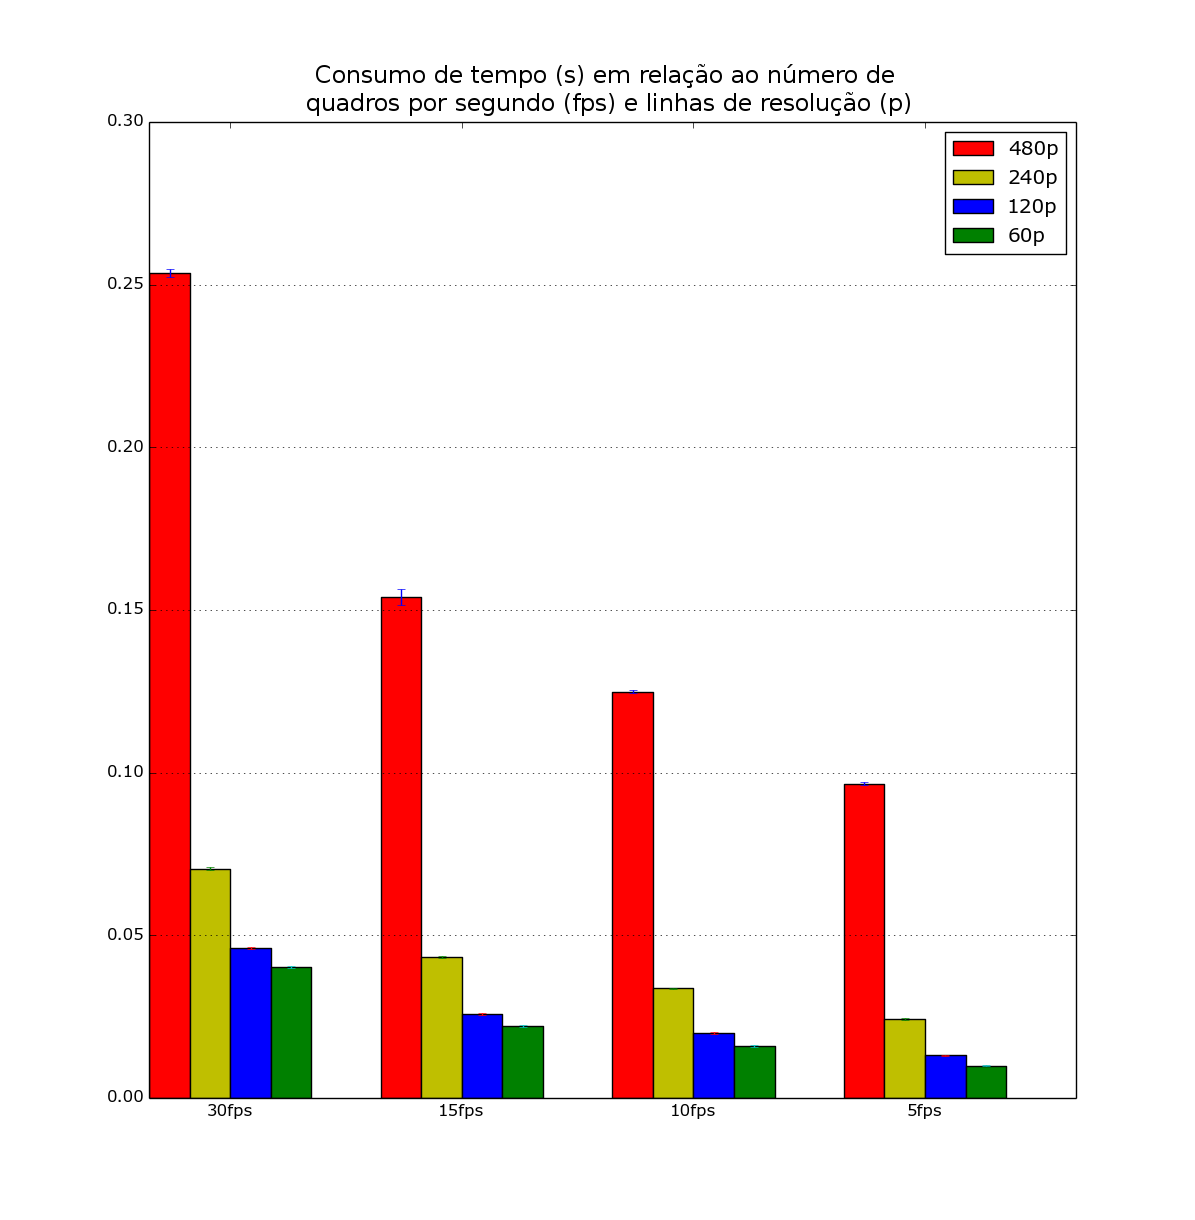
\includegraphics[width=13cm]{imgs/lowpower.png}
			\caption{\footnotesize {Relação entre consumo de CPU (em segundos) e o número de linhas de resolução. Com 240 linhas, há um ótimo custo-benefício entre redução de processamento e acurácia.}}
			\label{fig:lowpower}
			\vspace{5mm}
		\end{figure}  
		
		%------------------------------------------------------------
		\subsection{Estudo dos algoritmos e a amostragem}
		Quando analisamos os três algoritmos da literatura para detecção de leitura \cite{Campbell-2001, Buscher-2008, Kollmorgen-2007}, logo notamos uma abordagem comum para reconhecimento de eventos do olhar --- em particular, das fixações.
		
		Essa metodologia parece bastante razoável quando a limitação de amostras não é um problema. Mas se pretendemos utilizar tais algoritmos em condições críticas, isto é, em que o consumo de energia deve ser o mínimo aceitável, não podemos supor que teremos uma quantidade suficiente de amostras para representar esses eventos.
		
		Considere, por exemplo, um rastreador que funcione a 5 Hz (em contraste com os comumente empregados, de 50 - 60 Hz). Isso significa que teremos uma amostra a cada 200 ms, o que nos garante, aproximadamente, apenas um ponto para cada fixação ocorrida durante a leitura de um texto. Nesse caso, como seria possível, por exemplo, distinguir uma fixação de um movimento de perseguição feito na mesma direção (Figura \ref{fig:aliasing_leitura}) e evitar o \textit{aliasing}?
		
		\begin{figure}[!ht]
			\centering
			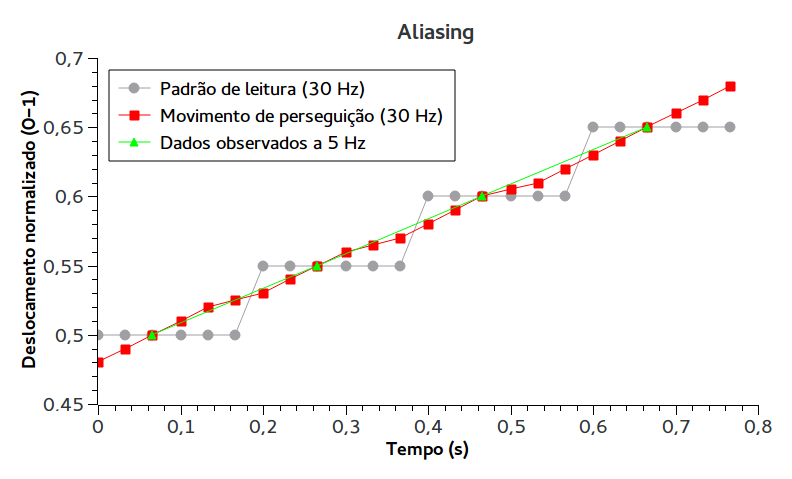
\includegraphics[width=14cm]{imgs/aliasing_leitura.png}
			\caption{\footnotesize {Exemplo de efeito de \textit{aliasing} a 5 Hz: o conjunto de fixações que define um padrão de leitura passa a ser indistinguível de um movimento de perseguição com a mesma direção e duração.}}
			\label{fig:aliasing_leitura}
			\vspace{5mm}
		\end{figure}
		
		Desde já, podemos intuir por que os algoritmos aqui abordados falham. Campbell e Maglio propõem uma filtragem dos dados por suavização \cite{Campbell-2001}, enquanto Buscher et al. e Kollmorgen e Holmqvist, cada qual à sua maneira, propõem uma interpretação de fixações em função de \textit{clusters} de pontos\cite{Buscher-2008, Kollmorgen-2007}. Em todos os casos, simplesmente não há pontos suficientes para a tarefa a 5 Hz.
		
		Na próxima seção, exibimos uma solução para esse problema e um comparativo entre alguns dos algoritmos e a nossa proposta. A chave para resolver o impasse, dado que a frequência de Nyquist não pode ser ignorada, está no fato de que não precisamos reconstruir um sinal digital em sua integridade para reconhecer o processo de leitura.  
		
		\clearpage
	%================================================================	
	\section{Novo algoritmo}
		
		%------------------------------------------------------------
		\subsection{Concepção e ideias centrais}
		Como não foi possível adaptar nenhum dos algoritmos na literatura para condições de baixa taxa de amostragem ($<$ 30 Hz), verificou-se a necessidade de desenvolver uma nova solução cujo principal atributo fosse a manutenção do desempenho no reconhecimento da leitura em diferentes frequências.
		
		Desse modo, procurou-se compreender que tipo de informação poderia ser preservada do olhar nessas condições e como seria possível traduzi-la para o padrão de leitura. A resposta veio com o processamento do sinal via quocientes diferenciais e o uso de uma máquina de estados.
		
		O quociente diferencial (ou \textit{quociente de Newton}) \cite{Belding-2008} é uma técnica bastante empregada no cálculo do que se costuma denominar em alguns meios como ``derivada discreta'' de uma função. A diferença entre ambos, porém, está no fato de que o conceito do quociente não implica obrigatoriamente que o denominador \textit{h}, na fórmula abaixo, tenda a zero: 
		
		$$\Delta f = \frac{f(x + h) - f(x)}{h}, \hspace{1cm}h > 0$$
		
		No caso do algoritmo proposto, o quociente é empregado como uma espécie de filtragem entre duas amostras consecutivas do olhar coletadas pelo rastreador. Como essas amostras são armazenadas digitalmente como pontos num espaço euclidiano discreto (e.g., a matriz que define a tela de um computador), ao aplicarmos o quociente entre dois pontos, obtemos a informação sobre direção, intensidade e deslocamento dos olhos em relação a uma superfície.
		
		Em outras palavras, se definirmos um espaço $\Delta f$ $\times$ \textit{amostras} (Figura \ref{fig:quociente}), perceberemos que, na ausência de movimento, $\Delta f$ tenderá a zero, enquanto que movimentos na direção crescente do espaço euclidiano discreto serão positivos e, na direção decrescente, negativos. Mais do que isso: se $\Delta f$ não depender do tempo, notaremos que os picos definidos pelos deslocamentos serão praticamente os mesmos, em termos de intensidade e direção, para diferentes taxas de amostragem. Nesse caso, o denominador $h$, constante, tem apenas o papel secundário de suavizar os dados.
		
		\begin{figure}[!ht]
			\centering
			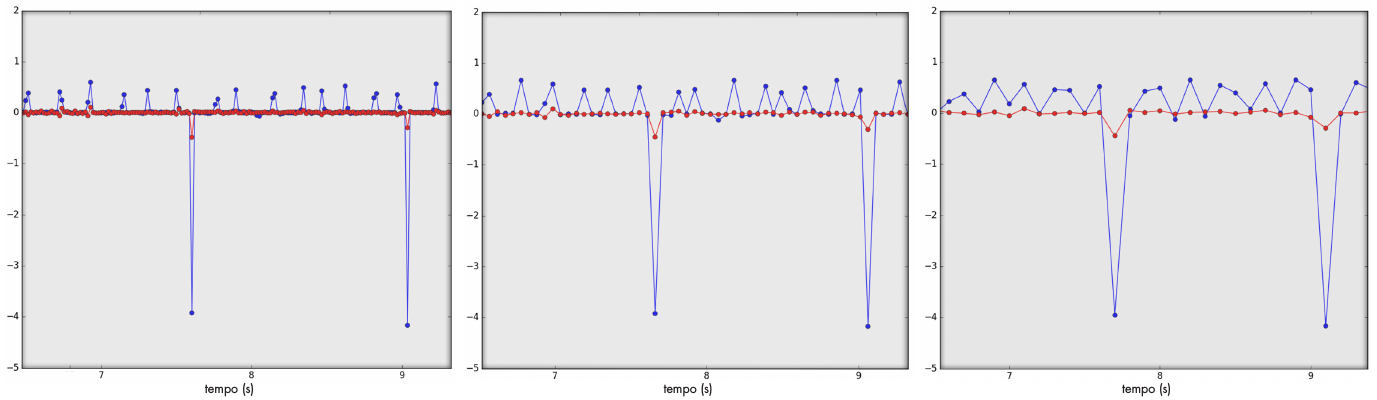
\includegraphics[width=16.5cm]{imgs/quocientes.png}
			\caption{\footnotesize {Da esquerda para a direita, o mesmo padrão de leitura amostrado em 30 Hz, 10 Hz e 5 Hz e exibido já com a transformação por quocientes diferenciais. Os pontos azuis correspondem a deslocamentos horizontais e os vermelhos, verticais.}}
			\label{fig:quociente}
			\vspace{5mm}
		\end{figure}
		
		Por outro lado, sem o uso de um mecanismo de validação de padrão, essa transformação por quocientes não impede que o algoritmo continue sujeito a \textit{aliasing}, dados anômalos ou falhas do rastreador. Assim, uma máquina de estados acaba se revelando bastante conveniente para o reconhecimento da leitura, visto que, uma vez verificado um determinado movimento por quocientes, ele só terá uma contribuição para o estado de detecção se estiver dentro de uma janela correta de movimentos. Dito de outra maneira, movimentos não associados à leitura ou aparentemente ruidosos, dentro de uma sequência de picos observados, reduzem o nível de evidências para o padrão.
		
		Para o algoritmo proposto, utilizamos uma janela de três quocientes calculados --- motivada por observações empíricas --- de modo que a cada nova configuração de janela, verificamos sua adequação à máquina de estados. Considerando como um evento todo quociente diferencial associado a uma sacada, os possíveis eventos observados pela máquina são as sacadas curtas realizadas à direita e as sacadas longas de regressão, feitas à esquerda. Desse modo, toda mudança de estado mapeada pelo diagrama da Figura \ref{fig:maquina} resulta em um incremento de evidências para a leitura e toda mudança não mapeada promove um decréscimo.
		
		\begin{figure}[!ht]
			\centering
			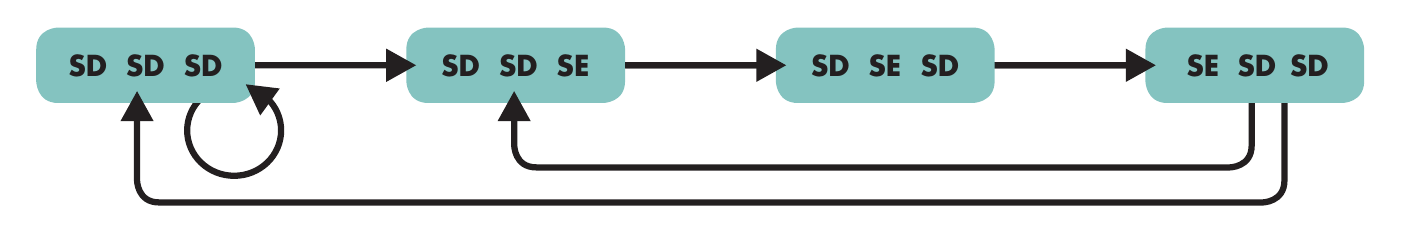
\includegraphics[width=16.5cm]{imgs/maquina_estados.png}
			\caption{\footnotesize {Grafo das transições de estado válidas para a leitura. A sigla \textbf{SD} indica uma sacada curta à direita e a sigla \textbf{SE}, uma regressão longa (que sinaliza mudança de linha).}}
			\label{fig:maquina}
			\vspace{5mm}
		\end{figure}
		
		Além disso, para caracterizar o \textit{skimming}, utilizamos o fato --- posteriormente confirmado em testes --- de que leitores rápidos tendem a fazer menos fixações por linha (Figura \ref{fig:skimming}), mas, ainda assim, realizando longas regressões à esquerda. Isso possibilitou que o algoritmo também pudesse se portar como um classificador não supervisionado do comportamento de leitura do usuário.
		
		\begin{figure}[!ht]
			\centering
			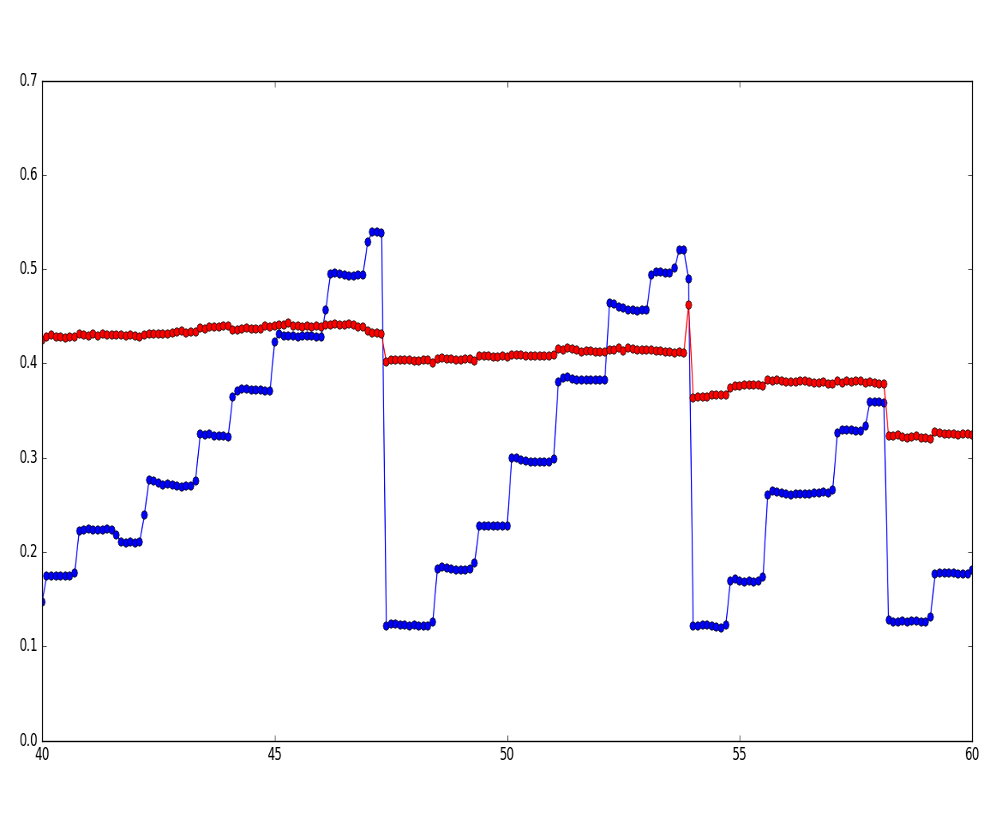
\includegraphics[width=7.8cm]{imgs/leitura_skimming1.png}
			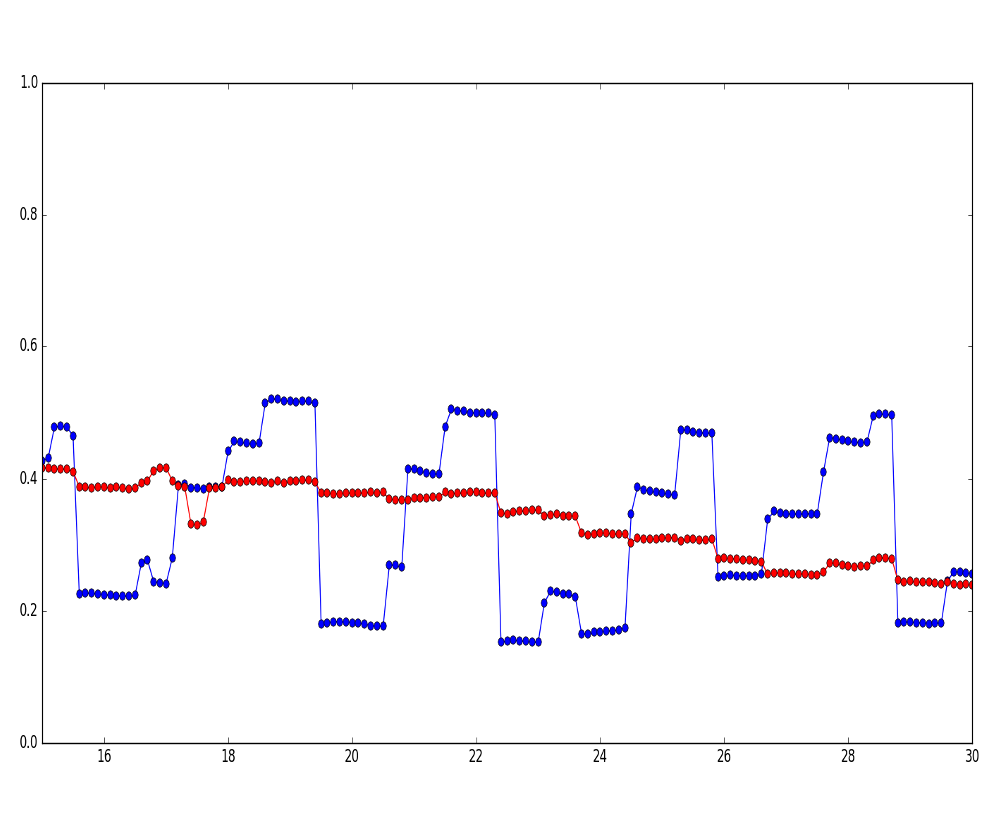
\includegraphics[width=7.8cm]{imgs/leitura_skimming2.png}
			\caption{\footnotesize {Comparação entre o padrão de leitura (esquerda) e o \textit{skimming} (direita) de um mesmo indivíduo. Note que no segundo caso, ainda que seja possível identificar um certo ``padrão de escadas'', o número de fixações por linha é significativamente menor.}}
			\label{fig:skimming}
			\vspace{5mm}
		\end{figure}
		
		
		%------------------------------------------------------------
		\subsection{Implementação}
		O algoritmo desenvolvido alterna indefinidamente entre dois ciclos: coleta dos dados do olhar e processamento dessas informações. Na fase de coleta, verifica-se a integridade e correção dos valores amostrados, uma vez que os pontos capturados pelo rastreador devem estar mapeados para dimensões válidas de uma superfície. Na fase de processamento, aplicam-se as técnicas de transformação, validação de janelas e classificação do estado de leitura.
		
		A alternância dos ciclos é definida por uma variável de condição, já que ambas as etapas são executadas em \textit{threads} distintas para se evitar o bloqueio da computação por problemas na captura de dados do rastreador.
		
		O cerne do algoritmo (Figura \ref{fig:algoritmo}) está no ciclo de processamento dos pontos do olhar e compreende os seguintes estágios: cálculo do quociente diferencial entre a amostra atual e a anterior --- tanto para o eixo das ordenadas quanto das abscissas ---, análise do quociente calculado, validação de janelas e verificação do estado de leitura.
		
		Na fase de análise do quociente, procura-se atestar se um pico calculado recai sobre uma faixa de valores válidos ou ultrapassa um determinado limiar. Em outras palavras, deseja-se encontrar sacadas curtas, regressões ou fixações a partir das transformações aplicadas.
		
		\begin{figure}[!ht]
			\centering
			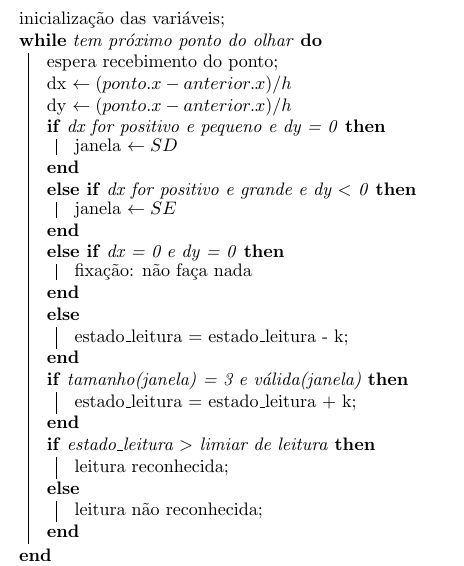
\includegraphics[width=10cm]{imgs/algoritmo.png}
			\caption{\footnotesize {Pseudocódigo que ilustra o ciclo de reconhecimento de leitura do algoritmo.}}
			\label{fig:algoritmo}
			\vspace{5mm}
		\end{figure}
		
		Já na fase de validação de janelas, acumula-se em uma variável a pontuação recebida por transições válidas de estado. Todavia, se a janela contiver movimentos não relacionados à leitura, essa variável sofre penalizações. Portanto, ao final do ciclo do algoritmo, se a pontuação acumulada for superior a um certo limiar, o algoritmo conclui que o indivíduo está lendo. 
		
		Opcionalmente, pode-se procurar ainda classificar o tipo de leitura do usuário (e.g., \textit{skimming} ou não), atribuindo-se uma pontuação com base no número de fixações por linha, o que pode ser verificado sempre que a máquina de estados completar um caminho do tipo \textit{SD SD SD} $\rightarrow$ \textit{SD SD SE} $\rightarrow$ \textit{SD SE SD} $\rightarrow$ \textit{SE SD SD}.
	
		
		
		%------------------------------------------------------------
		\subsection{Testes e metodologia}
		Para aferir o desempenho do algoritmo proposto, realizamos um experimento de leitura que contou com nove indivíduos --- cinco homens e quatro mulheres. Os textos selecionados para os testes foram 15 biografias em domínio público (entre 120 e 170 palavras) de cientistas e artistas célebres. Já como protocolo de controle, selecionamos 10 imagens, também em domínio público, contendo objetos repetidos.
		
		\begin{figure}[!ht]
			\centering
			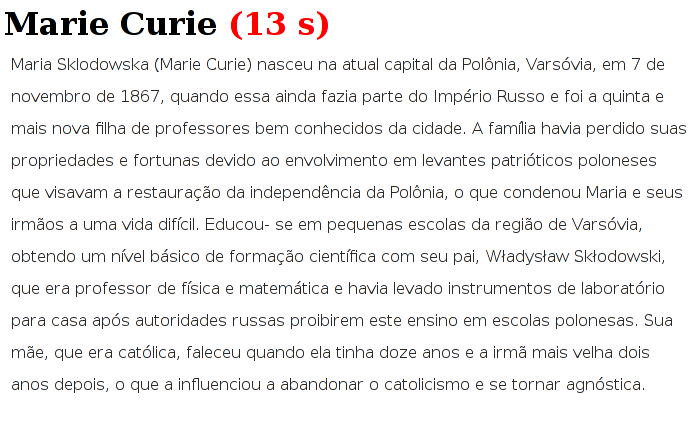
\includegraphics[width=7.8cm]{imgs/experimento1.png}
			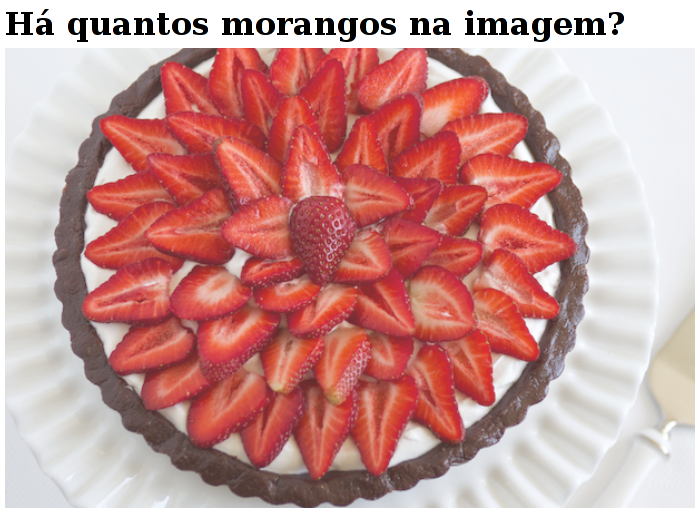
\includegraphics[width=7.8cm]{imgs/experimento2.png}
			\caption{\footnotesize {Dois exemplos da interface gráfica utilizada no experimento. À esquerda, um texto para \textit{skimming}, que deveria ser lido em até 13 segundos. À direita, uma imagem com objetos que deveriam ser contados pelos participantes.}}
			\label{fig:experimento}
			\vspace{5mm}
		\end{figure}
		
		Para cada participante foi exibida uma sequência aleatória contendo cinco textos para serem lidos em velocidade normal, cinco em velocidade rápida e cinco imagens. Todos os textos e imagens, por sua vez, também foram selecionados aleatoriamente. Exemplos desse material podem ser vistos na Figura \ref{fig:experimento}.
		
		Quando um texto era exibido ao usuário, este deveria lê-lo por completo e logo depois responder um questionário com três perguntas de múltipla escolha para avaliar o seu grau de compreensão (apenas para efeito de controle). No caso de textos para leitura rápida, o usuário deveria procurar extrair o máximo possível de informações, mesmo que não conseguisse concluir sua leitura, dado que havia um limite de tempo, e, em seguida, responder o mesmo tipo de questionário. Já para as imagens, a tarefa requisitada foi a contagem de objetos presentes e, nesse caso, o usuário deveria registrar o valor que contabilizou. 
		
		A tarefa de contagem de objetos em imagens foi definida dessa forma em razão da hipótese de que os movimentos realizados nesse caso seriam uma alternância entre fixações e sacadas curtas, tal qual na leitura, mas sem um padrão característico. Já os limites de tempo para a tarefa de \textit{skimming} foram motivados pela literatura \cite{Dyson-2001}.
		
		Todos os dados foram coletados a 30 Hz, utilizando-se o \textit{Pupil Eye Tracker}, e posteriormente subamostrados para 10 Hz e 5 Hz, o que totalizou 45 amostras de leitura, 45 de \textit{skimming} e 45 de imagens (controle) para cada faixa de frequência. 
		
		A partir dessas informações, procuramos avaliar a especificidade e a sensibilidade do algoritmo proposto em comparação com os trabalhos de Buscher et al. \cite{Buscher-2008} e Campbell e Maglio \cite{Campbell-2001}, referências encontradas na literatura para reconhecimento de leitura em tempo real. Já para o padrão de \textit{skimming}, apenas procuramos mensurar os resultados obtidos no experimento.
		
		%------------------------------------------------------------
		\subsection{Resultados}
		Para cada um dos algoritmos, foram avaliadas a taxa de acerto (sensibilidade) e a taxa de verdadeiros negativos (especificidade). O teste de Kolmogorov-Smirnov mostrou que os dados seguem uma distribuição normal para um $p < 0.05$. Assim, visto que a variância da população era desconhecida, calculamos a média das duas medidas para um intervalo de confiança de 95\% bicaudal, utilizando a distribuição t de Student.
		
		A sensibilidade foi definida como o usual, isto é, o número de verdadeiros positivos (VP) detectados pelo algoritmo sobre o total de verdadeiros positivos na amostra, o que inclui dados não detectados (FN):
		
		$$Sensibilidade = \frac{VP}{VP + FN}$$
				
		A especificidade, por sua vez, foi definida como o número de dados não relacionados à leitura (VN) reconhecidos pelo algoritmo sobre o total de verdadeiros negativos na amostra, o que inclui dados erroneamente classificados como de leitura (FP):
		
		$$Especificidade = \frac{VN}{VN + FP}$$
		
		Já as amostras de \textit{skimming} se mostraram inconclusivas para efeito de avaliação, visto que a maioria dos participantes não seguiu o protocolo definido, a ponto de muitos terem lido os textos para esse propósito com quase a mesma velocidade desempenhada na leitura convencional. Em função disso, as Figuras \ref{fig:sensibilidade} e \ref{fig:especificidade} relatam apenas os resultados obtidos sem o classificador de \textit{skimming}.
		
		\begin{figure}[!ht]
			\centering
			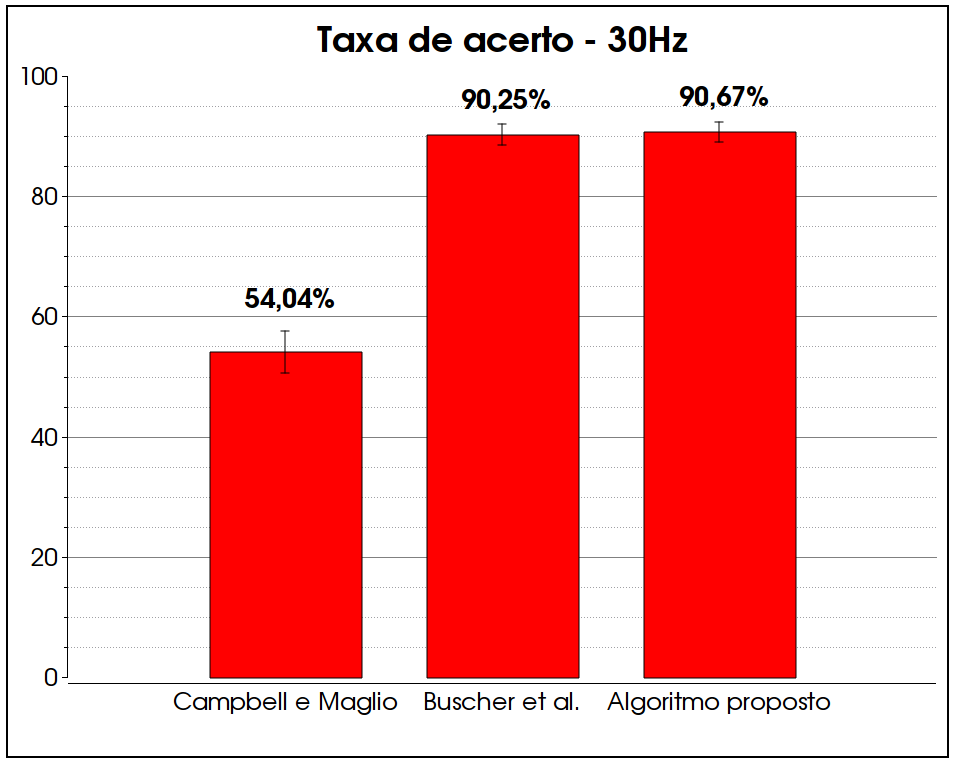
\includegraphics[width=7.85cm]{imgs/Graph1.png}
			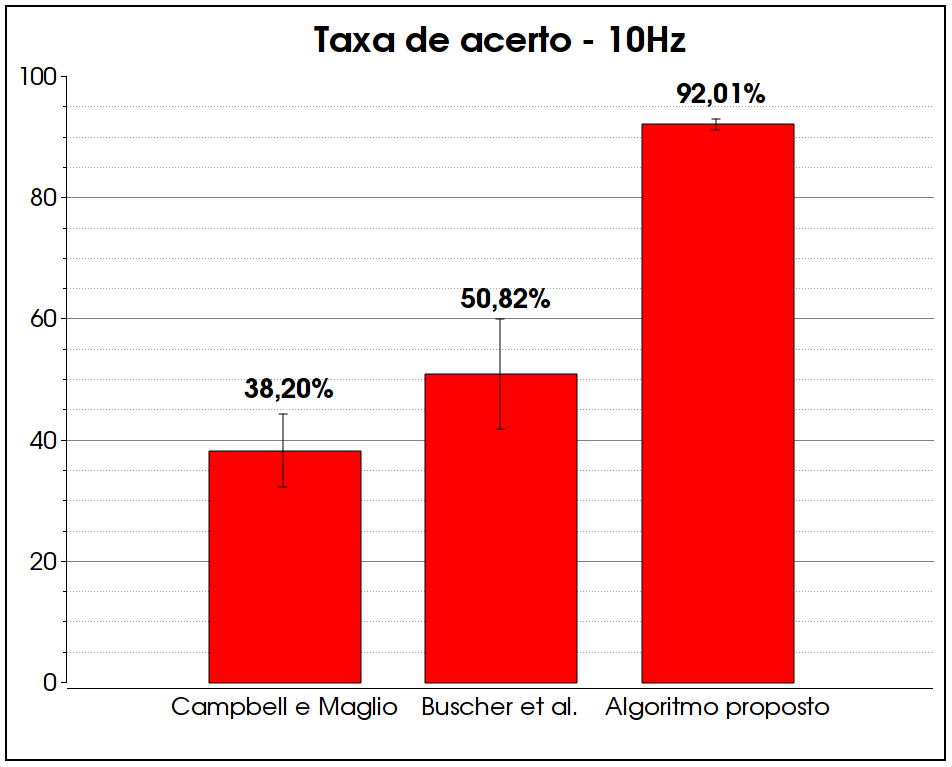
\includegraphics[width=7.85cm]{imgs/Graph2.png}
			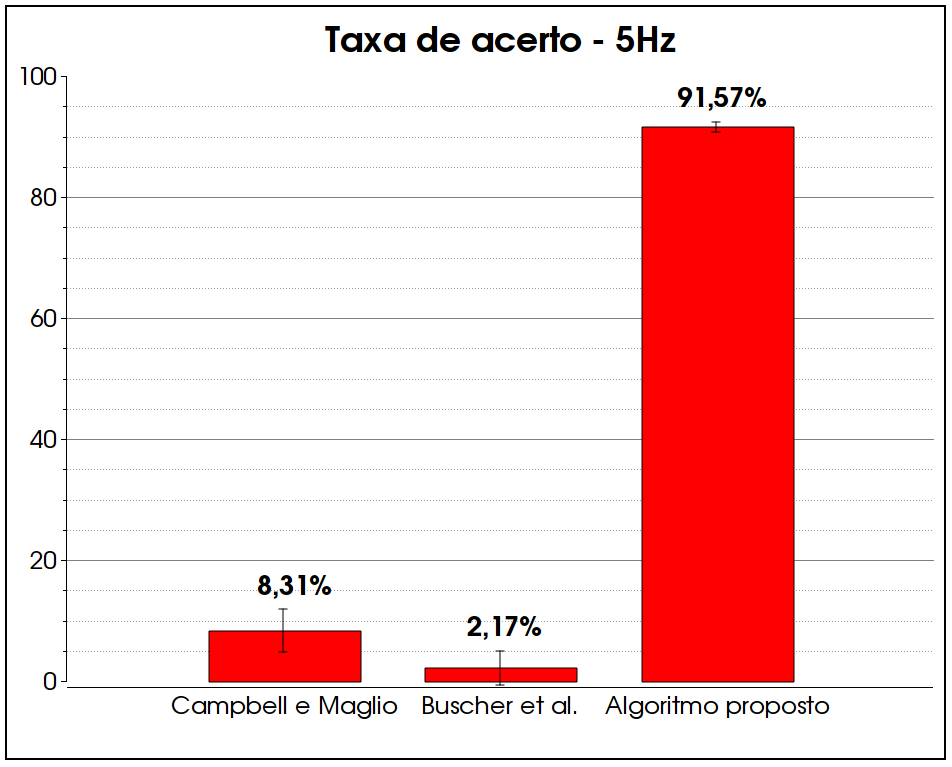
\includegraphics[width=7.85cm]{imgs/Graph3.png}
			\caption{\footnotesize {Comparação de sensibilidade em três diferentes frequências para os algoritmos de Campbell e Maglio (2001), Buscher et al. (2008) e o desenvolvido neste trabalho.}}
			\label{fig:sensibilidade}
			\vspace{5mm}
		\end{figure}
		
		\begin{figure}[!ht]
			\centering
			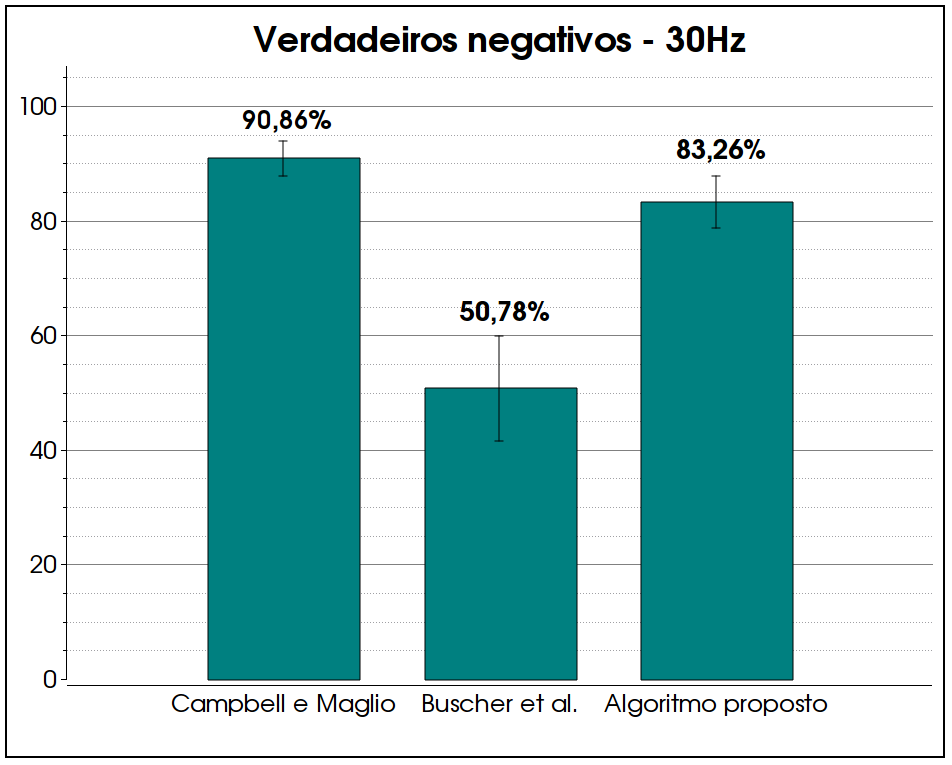
\includegraphics[width=7.85cm]{imgs/Graph4.png}
			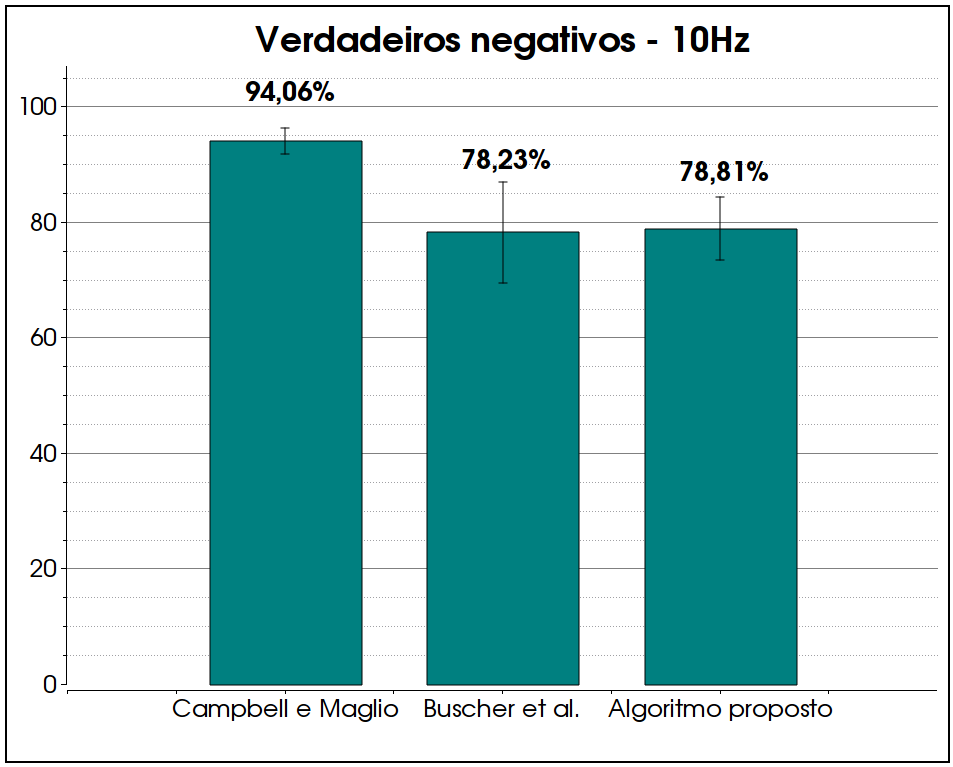
\includegraphics[width=7.85cm]{imgs/Graph5.png}
			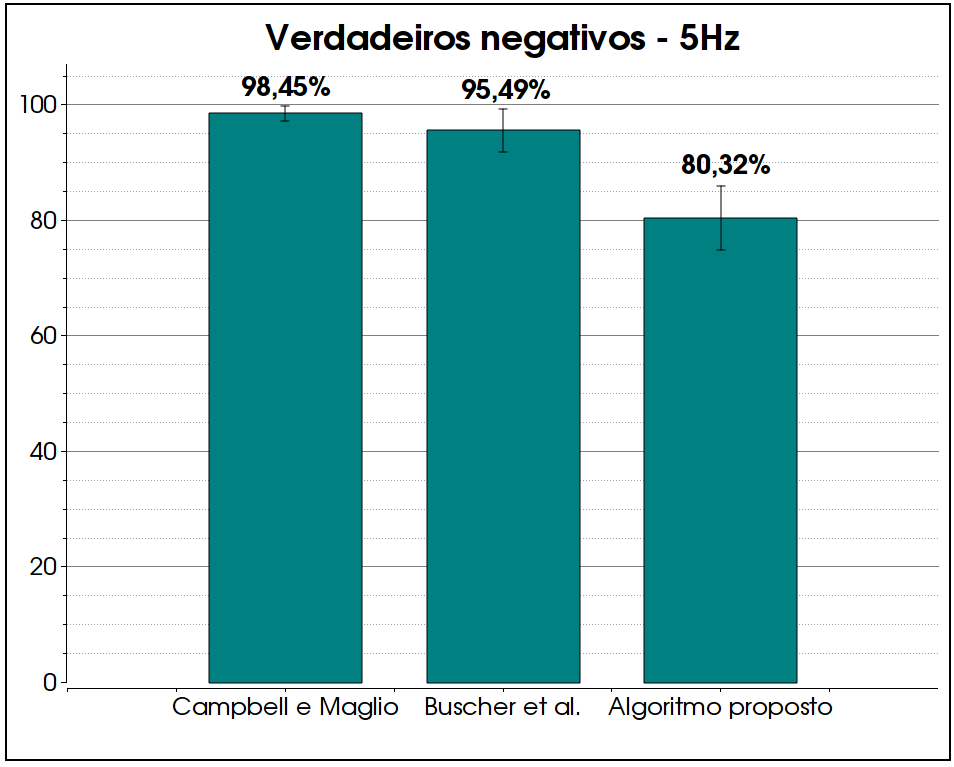
\includegraphics[width=7.85cm]{imgs/Graph6.png}
			\caption{\footnotesize {Comparação de especificidade em três diferentes frequências para os algoritmos de Campbell e Maglio (2001), Buscher et al. (2008) e o desenvolvido neste trabalho.}}
			\label{fig:especificidade}
			\vspace{5mm}
		\end{figure}
		
		%------------------------------------------------------------
		\subsection{Discussão}
		O algoritmo proposto mostrou um desempenho geral bastante satisfatório em comparação com os demais. Em termos de sensibilidade (Figura \ref{fig:sensibilidade}), a taxa de acerto foi um pouco superior a 90\% em todas as amostragens, o que demonstra a capacidade do algoritmo de manter um patamar de desempenho independentemente da frequência. Um cenário semelhante também foi observado em relação à taxa de falsos negativos, em que nota-se um desempenho estável na faixa de 80\% para todas as frequências.
		
		Em relação aos acertos, podemos verificar que a técnica dos quocientes garante à máquina de estados o reconhecimento do padrão de leitura, como era esperado. Já para os demais algoritmos, vemos uma clara queda de desempenho com a redução da frequência, o que é ainda mais acentuado no caso de Buscher et al. do que no de Campbell e Maglio. Uma explicação para isso está no fato de que o algoritmo de Buscher et al. precisa reconhecer fixações antes de analisar o movimento realizado, o que demanda um processo de \textit{clustering} de muitos pontos, enquanto que o algoritmo de Campbell e Maglio parece apresentar deficiências no seu modelo de leitura.
		
		Quanto aos verdadeiros negativos (Figura \ref{fig:especificidade}), pode-se observar que embora o algoritmo proposto tenha se mostrado estável e relativamente satisfatório em todas as frequências, ainda assim, tanto o algoritmo de Campbell e Maglio quanto o de Buscher et al. exibiram um ganho de desempenho proporcional à diminuição da taxa de amostragem. 
		
		Há pelo menos duas explicações para isso. A primeira é a de que a taxa de verdadeiros negativos não corresponde, necessariamente, a um comportamento acurado ótimo quando os algoritmos em questão também perdem a capacidade de reconhecer verdadeiros positivos. Em outras palavras, um classificador com 100\% de especificidade é irrelevante se apresenta 0\% de sensibilidade.
		
		A segunda explicação está no fato de que muitos indivíduos, em alguns momentos, realizaram a contagem de objetos nas tarefas com imagens como se estivessem, de fato, lendo, isto é, movimentando seus olhos de modo a emular quase que perfeitamente o padrão de leitura, fato que acabou se mostrando recorrente para algumas das imagens selecionadas. Os usuários que, em geral, não contaram objetos dessa maneira exibiram um nível de especificidade superior a 90\% para o algoritmo proposto.
		
		Quanto ao classificador de \textit{skimming}, os experimentos revelaram não apenas a impossibilidade de avaliar o trabalho desenvolvido, como também o fato do comportamento de leitura de alguns participantes ser equiparável ao de \textit{skimming} de outros, isto é, constatou-se que algumas pessoas liam, na sua cadência normal, a uma velocidade considerada muito rápida para outras. Com isso, a hipótese de que seria possível criar um classificador não supervisionado de \textit{skimming} genérico mostrou-se incompatível com as observações empíricas. Contudo, o desenvolvimento de um classificador adaptado aos padrões de cada indivíduo ainda mostra-se factível.
		
		    
		
		
		\clearpage
	%================================================================
	\section{Prova de conceito}
	
		%------------------------------------------------------------
		\subsection{Idealização}
		A ideia de uma prova de conceito (PoC) para o projeto surgiu da percepção de que a pesquisa realizada com algoritmos para reconhecimento de leitura necessitava de uma ponte para algumas das questões que motivaram o trabalho, como aplicações capazes de melhorar a qualidade das interações dos usuários e, ao mesmo tempo, consumir pouca energia.
		
		Inicialmente, cogitou-se o desenvolvimento de uma prova de conceito para \textit{smart glasses}, mas dada a indisponibilidade de uma arquitetura com rastreadores de olhar associados a \textit{displays} vestíveis, essa possibilidade, embora ideal para os propósitos do projeto, gradualmente mostrou-se inexequível.
		
		Desse modo, os esforços iniciais foram subdimensionados para uma arquitetura convencional, mas genérica o bastante para permitir fácil adaptação e distribuição em diferentes plataformas. Utilizamos, então, a tela comum do computador como superfície de mapeamento dos movimentos oculares e eliminamos a necessidade do reconhecimento ótico de caracteres via imagem da cena.
		
		A PoC consiste em utilizar o reconhecimento do padrão de leitura como mecanismo mediador de interações, que podem ser segmentadas em duas classes: convencional e aumentada. Se o algoritmo não detecta um estado de leitura, o sistema permite que o usuário realize suas tarefas típicas. Caso contrário, interrupções indesejadas, tais como notificações de sistema, mensagens, notícias, entre outras, são temporariamente bloqueadas para que o usuário possa desempenhar sua atividade primária (leitura). 
		
		No caso do reconhecimento do estado de leitura, afirmamos que a classe de interação é \textit{aumentada} porque a experiência da leitura pode ser melhorada com recursos de apoio \cite{Biedert-2010}, como gráficos, sons, sugestões de conteúdos relacionados, marcação automática de páginas, traduções de termos estrangeiros, entre outras possibilidades.		
		
		
		%------------------------------------------------------------
		\subsection{Descrição do software}
		A plataforma escolhida para o desenvolvimento da prova de conceito foi o \textit{Google Chrome}, em particular, por sua ubiquidade, facilidade de uso e popularidade.
		
		O \textit{software} consiste em uma extensão para o navegador da Google capaz de se comunicar com um servidor \textit{WebSockets} que, por sua vez, disponibiliza dados coletados do olhar. A extensão processa esses dados por meio do algoritmo proposto de reconhecimento de leitura e, caso a detecte, sinaliza a mudança de estado por meio de um ícone na janela do navegador (Figura \ref{fig:pocface1}).
		
		\begin{figure}[!ht]
			\centering
			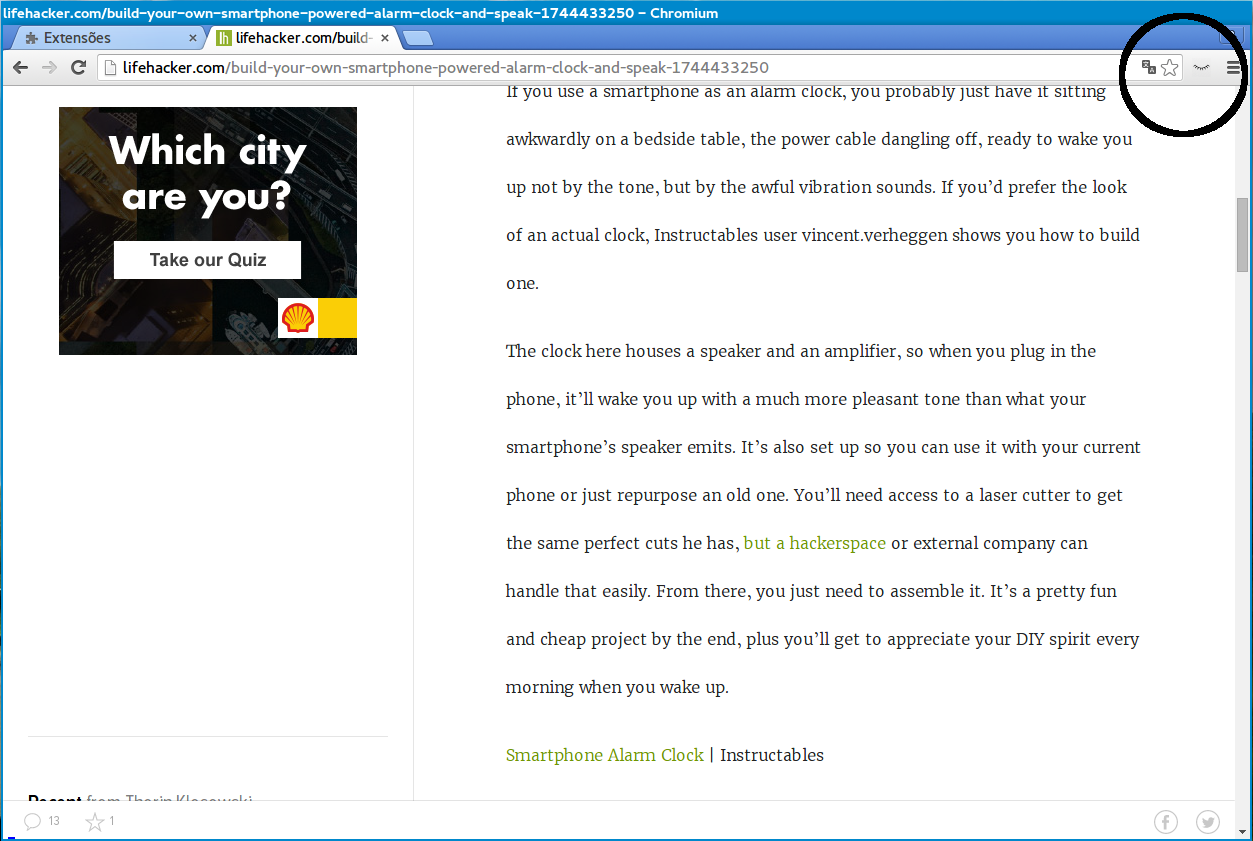
\includegraphics[width=7.8cm]{imgs/poc_fechado.png}
			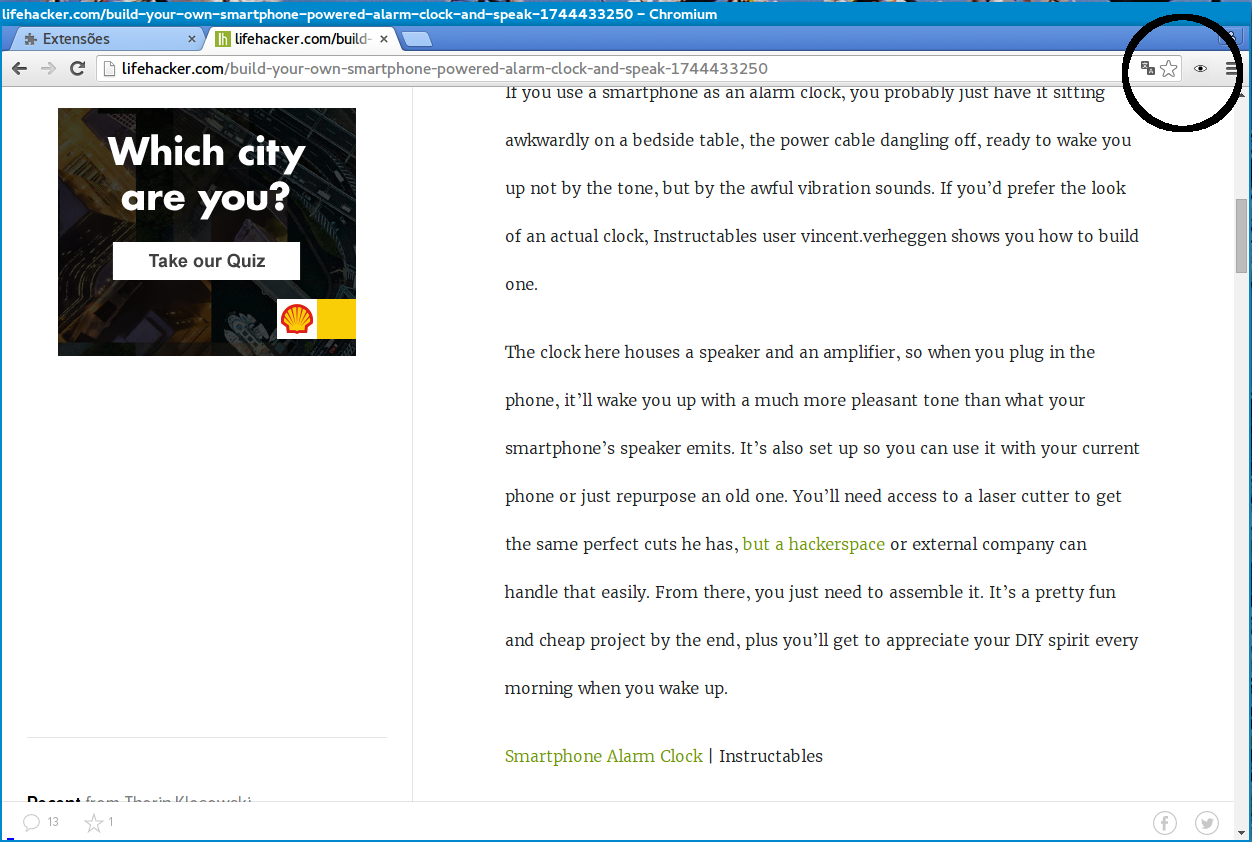
\includegraphics[width=7.8cm]{imgs/poc_aberto.png}
			\caption{\footnotesize {À direita, o ícone de um olho fechado (canto superior direito) indica que o padrão de leitura ainda não foi detectado. À esquerda, o ícone é trocado pelo desenho de um olho aberto, dando \textit{feedback} de que a atividade de leitura foi reconhecida.}}
			\label{fig:pocface1}
			\vspace{5mm}
		\end{figure}
		
		
		Com a ativação da extensão, duas tarefas de pré-processamento são realizadas sobre as páginas HTML do navegador: o aumento do entrelinhamento dos textos, a fim de evitar problemas associados à acurácia limitada dos rastreadores, e a ``tokenização'' de cada palavra no corpo da página mediante encapsulamento por \textit{tags}, com o intuito de descobrir em que coordenada da tela um termo se encontra e, dessa forma, relacioná-lo à posição do olhar.
		
		Os recursos de aumento da interação implementados foram um marcador do último ponto de parada da leitura, a autorrolagem --- para permitir interações sem as mãos --- e a tradução de palavras de origem inglesa (Figura \ref{fig:pocface2}), que é ativada sempre que o usuário fixar-se temporariamente em um termo por cerca de dois segundos durante a leitura.
		
		\begin{figure}[!ht]
			\centering
			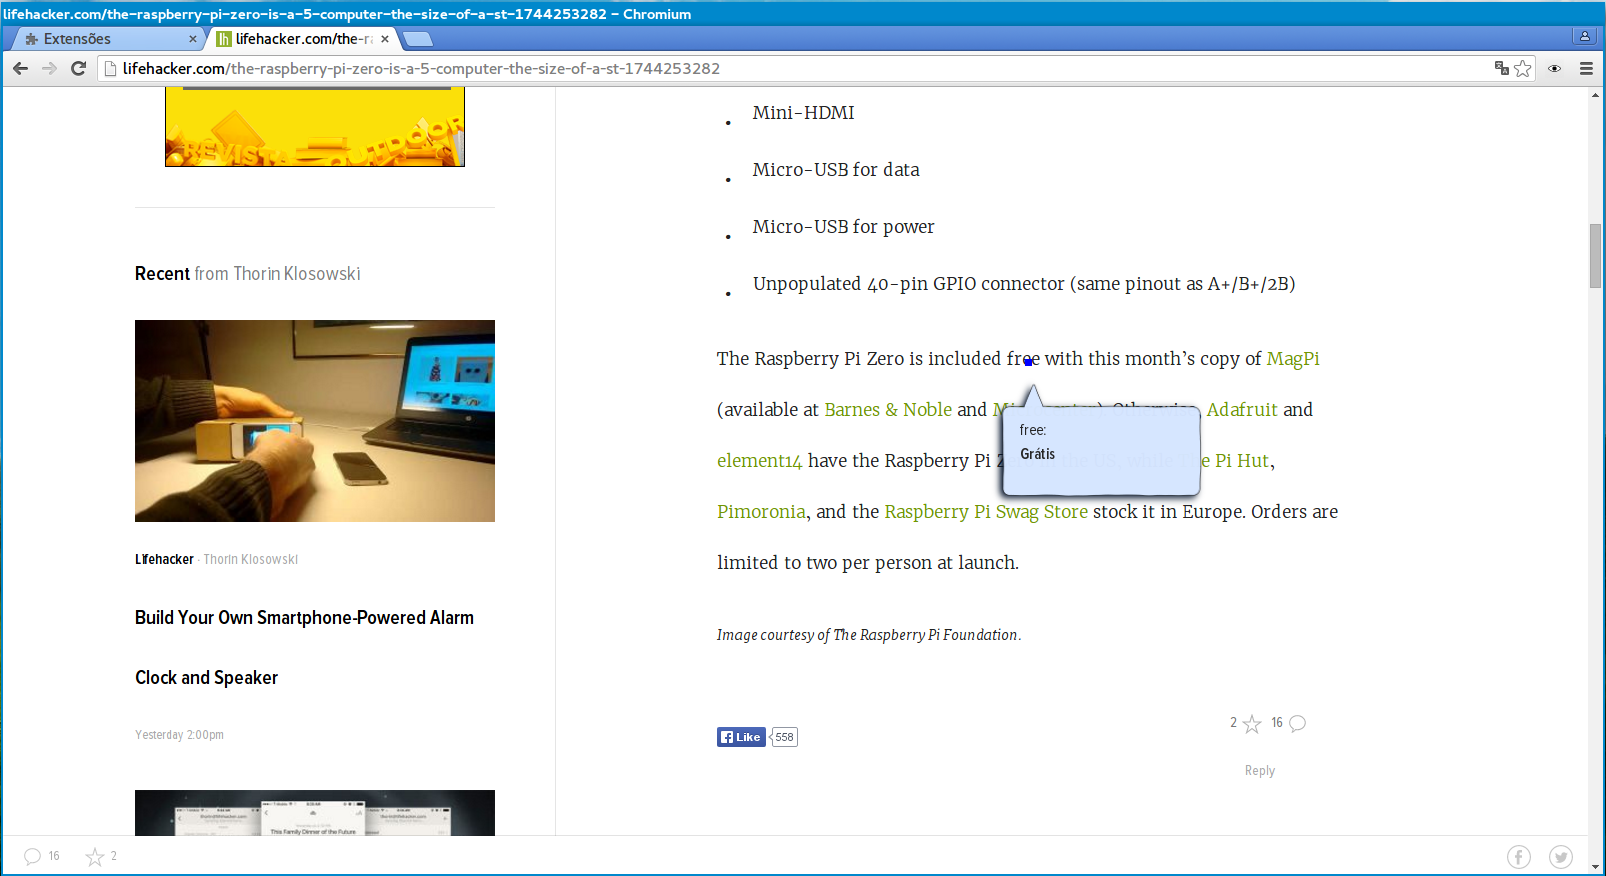
\includegraphics[width=16cm]{imgs/poc_balao.png}
			\caption{\footnotesize {Exemplo de aumento da experiência de leitura: fixações longas em um termo de origem inglesa ativam um sistema de busca pela tradução da palavra para a língua portuguesa.}}
			\label{fig:pocface2}
			\vspace{5mm}
		\end{figure}
		
		

		
		
		\clearpage
	%================================================================
	\section{Conclusões}
	
		%------------------------------------------------------------
		\subsection{Eliminando os problemas da baixa taxa de amostragem}
		Do ponto de vista do desenvolvimento de algoritmos, este trabalho procurou demonstrar que, embora não seja possível oferecer soluções genéricas para problemas associados à baixa frequência, em alguns casos é perfeitamente viável oferecer saídas satisfatórias para problemas particulares.
		
		O reconhecimento da leitura acabou se mostrando um exemplo disso. Se por um lado, questões inerentes à baixa taxa de amostragem --- tais como \textit{aliasing} e anomalias --- são inevitáveis, por outro, essas questões não configuram necessariamente um impedimento para atingir um fim desejado.
		
		A chave encontrada no projeto para solucionar essas dificuldades estava justamente em olhar lateralmente para o problema e verificar que não é necessário resolver questões intermediárias se podemos, de outra maneira, solucionar as questões que realmente importam para os nossos propósitos.
		
		O recurso lateral, no nosso caso, foi utilizar uma máquina de estados que pudesse interpretar um comportamento já extensivamente estudado na literatura. Mas trata-se de uma solução \textit{ad-hoc}, que embora possa oferecer alguma inspiração para resolver outros problemas associados à baixa taxa de amostragem, certamente não pode ser generalizada.
		
		%------------------------------------------------------------
		\subsection{Comunicação passiva como forma de interação}
		Tanto na literatura quanto nos dispositivos disponíveis para consumo massivo, há uma clara opção pelo uso de interfaces baseadas em seleção. Contudo, nas mais diversas atividades cotidianas, interações dessa forma, em que o usuário tradicionalmente emprega suas mãos para ativar algum recurso do sistema, nem sempre são possíveis.
		
		O uso do olhar é uma alternativa a ser considerada nesses casos, visto que é possível depreender vários aspectos do comportamento e da intenção do usuário a partir dos movimentos oculares. Em particular, certos padrões na leitura são muito proveitosos para predições de níveis de interesse, como já mencionado em seções anteriores.
		
		A prova de conceito desenvolvida para este projeto procurou demonstrar que a leitura é uma das atividades que podem ser empregadas como mecanismo passivo de interação, seja para melhorá-la, como técnica mediadora, seja para substituir funcionalidades tipicamente associadas a comportamentos de seleção.
		
		No segundo caso, em que gestos deliberados e assertivos do usuário são trocados por gestos espontâneos, a expectativa é de que o indivíduo realize interações com menos esforços e mais simplicidade, o que, em tese, poderia lhe proporcionar ganhos de produtividade e conforto.
		
		%------------------------------------------------------------
		\subsection{Consumo de energia e questões em aberto}
		Os resultados deste trabalho atestam que um reconhecimento robusto da leitura é algo realizável a taxas de amostragem de 5 Hz, seis vezes a menos do que o regime convencional de funcionamento do rastreador utilizado nos testes. Com isso, seria possível conjecturar sobre um ganho de iguais proporções em economia de energia por meio de uma câmera de baixa frequência para o rastreamento da pupila.
		
		Além disso, o algoritmo apresentado demanda operações de baixo consumo de ciclos do processador (e.g., operações aritméticas simples) e tem complexidade linear no número de amostras --- ao contrário, por exemplo, do algoritmo de Buscher et al., de complexidade potencialmente quadrática \cite{Buscher-2008}.
		
		Entretanto, um dos entraves para que esses benefícios se tornem mensuráveis está na disponibilidade de \textit{hardware}, uma vez que a demanda sobre o consumo de energia só seria reduzida de fato com a oferta de câmeras de baixo desempenho e processadores otimizados para regimes de frequência reduzida.
		
		No caso da leitura, uma das dificuldades não abordados no projeto está em como prover uma experiência \textit{aumentada} na interação de modo a não prejudicar o usuário. O trabalho de Biedert et al. \cite{Biedert-2010} demonstra uma série de recursos que poderiam ser empregados para tornar a leitura de um livro mais rica, por exemplo, mas esses recursos, por vezes, podem ter um caráter intrusivo se o usuário não tiver condições optar ou não por sua ativação.
		
		Outros tópicos que mereceriam exploração são a questão da privacidade do usuário em meio à coleta de dados sobre o seu comportamento, o problema sobre que tipo de aumento é relevante durante a leitura ou ainda o impacto social dessa tecnologia em determinados nichos, como educação, saúde e segurança.
		
		
		 
        \clearpage

	%================================================================
	\section{Parte subjetiva}
	
		%------------------------------------------------------------
		\subsection{Dificuldades e frustrações}
		Uma das maiores dificuldades vividas neste projeto foi ter de andar por um terreno que considerei cientificamente obscuro. Quando meu orientador propôs o tema de trabalho, não sabia ainda que não havia absolutamente nada na literatura a respeito de algoritmos para padrões do olhar em baixa frequência.
		
		De certa forma, absorvi esse desafio como um voto de confiança e procurei me munir da maior quantidade possível de informações sobre o assunto: desde o \textit{hardware} do rastreador, passando por algoritmos de reconhecimento da pupila, processamento de sinais digitais, processos cognitivos, até chegar, finalmente, nos algoritmos para reconhecimento de leitura.
		
		Ao tentar adaptar os algoritmos para o problema da baixa taxa de amostragem, percebi que seria necessário ter um pouco de criatividade para resolvê-lo. Um dos principais entraves estava no fato de todos os algoritmos estudados se apoiarem apenas no processamento de sinais, o que se torna problemático em baixas frequências. Outra dificuldade estava em como fazer com que um sinal mostrasse uma assinatura semelhante em diferentes amostragens.
		
		Para atacar o último problema, comecei a pensar lateralmente e a ideia de limiares com quociente diferencial acabou tomando corpo e, felizmente, mostrou-se aplicável. Mas notei que apenas esse processamento não seria suficiente: a leitura tem um padrão característico, então por que não reconhecer o padrão em si em vez de limitar-se ao sinal? Com isso, o novo algoritmo ganhou vida.
		
		No início, quando verifiquei que minha solução estava se mostrando cada vez mais viável, minha ingenuidade me levou a cometer dois erros típicos relacionados a \textit{overfitting}: o primeiro deles foi acreditar que melhorar a acurácia do algoritmo indefinidamente não provocaria impacto algum sobre a taxa de falsos positivos. O segundo, foi acreditar que trabalhando com apenas dados de uma pessoa já seria possível adquirir evidências fortes o bastante para um bom comportamento do algoritmo. Essas fontes de frustrações, de certa maneira, converteram-se em lições valiosas para dar robustez ao trabalho.
		
		Outro problema ocorreu na fase de coleta de dados de voluntários. Como o protocolo acabou se revelando um pouco falho, acabei perdendo valiosas amostras e, de 13 participantes, quatro tiveram seus dados descartados. Pode não ter sido um desastre para o projeto, mas é inevitável não se sentir pesaroso por ter feito algumas pessoas doarem um tempo que não pôde ser aproveitado.
		
		Mas talvez a maior frustração tenha surgido na fase de desenvolvimento da prova de conceito. Isso porque, pelo meu planejamento inicial, a aplicação idealizada deveria funcionar, inclusive, para meios físicos, como textos impressos. Contudo, esse processo envolveria captação da imagem da cena por uma câmera de alta definição acoplada à cabeça do usuário, o processamento da imagem para reconhecimento de caracteres (OCR) e o emprego de um \textit{display see-through} para interações mediadas pelo algoritmo de leitura. 
		
		Tudo isso acabou se mostrando inviável, não apenas em função da falta de equipamentos, como também pela limitação técnica das câmeras e da qualidade de pacotes OCR abertos. Resultado: um mês de trabalho perdido e mais uma lição aprendida sobre viabilidade \textit{versus} prioridade.
		
		
		%------------------------------------------------------------
		\subsection{Disciplinas relevantes}
		No campo da teoria, acredito que as disciplinas mais relevantes para o trabalho foram as de Visão e Processamento de Imagens (MAC0417) e Cálculo Diferencial e Integral I (MAT0111), uma vez que foi com conceitos presentes nelas que o algoritmo deste projeto foi desenvolvido. Ainda assim, não poderia deixar de salientar a contribuição do meu projeto de Iniciação Científica (2014) para minha formação acadêmica, bem como da disciplina de Atividade Curricular em Pesquisa (MAC0215), que cumpriu o papel de me introduzir informalmente aos estudos em Interação Homem-Computador. 
		
		Já as disciplinas de estatística básica (MAE0121 e MAE0212) foram essenciais para o tratamento e a análise dos dados. Sem conceitos como independência das variáveis, significância estatística, normalidade, Teorema do Limite Central e tantos outros, não havia como ter confiança de que o trabalho estava sendo executado corretamente. Sem essas ferramentas, não seria possível justificar adequadamente um estudo não determinístico sem recorrer ao apelo à autoridade.
		
		As disciplinas práticas e de laboratório também tiveram sua contribuição para o trabalho, embora indireta, já que é nelas que desenvolvemos um raciocínio mais apurado para programação, aprendemos a depurar código e entendemos como integrar pedaços de \textit{software} distintos. Dado que a prototipagem rápida de interfaces e o uso dos mais diferentes equipamentos é um lugar comum na área de Interação Homem-Computador, o desenvolvimento do projeto sem essas habilidades se revelaria inviável. Em particular, acredito que merecem menção as disciplinas de Programação Concorrente (MAC0438), Programação para Redes (MAC0448) e Sistemas Operacionais (MAC0422).
		
		Penso ainda que seria injusto não creditar minha verdadeira estima à disciplina de Álgebra II (MAT0213), especialmente pela sua capacidade de insinuar uma nova forma de ver o mundo, de permitir reconhecer o valor do pensamento abstrato e de como resolver \textit{lateralmente} problemas aparentemente sem soluções.
		
		%------------------------------------------------------------
		\subsection{Projetos futuros}
		
		Em termos de atividade acadêmica, este trabalho poderá servir de insumo para uma futura publicação. Evidentemente, uma revisão mais crítica do projeto será necessária, bem como uma possível refatoração do protocolo experimental, sobretudo para a parte de classificação de leitura rápida ou convencional.
		
		Do ponto de vista da aplicação do trabalho, há a possibilidade de converter a prova de conceito desenvolvida aqui em um aplicativo de fato, particularmente, para dispositivos vestíveis, o que não se mostrou possível ao longo do projeto, devido às limitações de tempo e equipamentos.
		

		\clearpage
		
		
		\makeatletter
		\renewenvironment{thebibliography}[1]
		{\section{\bibname}% <-- this line was changed from \chapter* to \section*
			\@mkboth{\MakeUppercase\bibname}{\MakeUppercase\bibname}%
			\list{\@biblabel{\@arabic\c@enumiv}}%
			{\settowidth\labelwidth{\@biblabel{#1}}%
				\leftmargin\labelwidth
				\advance\leftmargin\labelsep
				\@openbib@code
				\usecounter{enumiv}%
				\let\p@enumiv\@empty
				\renewcommand\theenumiv{\@arabic\c@enumiv}}%
			\sloppy
			\clubpenalty4000
			\@clubpenalty \clubpenalty
			\widowpenalty4000%
			\sfcode`\.\@m}
		{\def\@noitemerr
			{\@latex@warning{Empty `thebibliography' environment}}%
			\endlist}
		\makeatother
		
	\bibliographystyle{plain}
	\bibliography{references} 

\end{document}